%% LyX 2.0.7 created this file.  For more info, see http://www.lyx.org/.
%% Do not edit unless you really know what you are doing.
\documentclass[amtd,hvmath]{copernicus_discussions}
\usepackage[T1]{fontenc}
\pagestyle{empty}
\usepackage{color}
\usepackage{verbatim}
\usepackage{float}
\usepackage{units}
\usepackage{graphicx}
\usepackage[authoryear]{natbib}
\PassOptionsToPackage{normalem}{ulem}
\usepackage{ulem}
\usepackage[unicode=true,pdfusetitle,
 bookmarks=true,bookmarksnumbered=false,bookmarksopen=false,
 breaklinks=false,pdfborder={0 0 0},backref=false,colorlinks=true]
 {hyperref}

\makeatletter

%%%%%%%%%%%%%%%%%%%%%%%%%%%%%% LyX specific LaTeX commands.
%% Because html converters don't know tabularnewline
\providecommand{\tabularnewline}{\\}

%%%%%%%%%%%%%%%%%%%%%%%%%%%%%% User specified LaTeX commands.
\usepackage{lineno}
%\linenumbers

\makeatother

\begin{document}



\title{Calibrating airborne measurements of airspeed, pressure and temperature
using a Doppler laser air-motion sensor}


\author{W. A. Cooper}


\author{S. M. Spuler}


\author{M. Spowart}


\author{D. H. Lenschow}


\author{R. B. Friesen}


\affil{National Center for Atmospheric Research, Boulder CO, U. S. A.}


\runningtitle{Calibrations with a laser air-motion sensor}


\runningauthor{W. A. Cooper et al.}


\correspondence{W. A. Cooper\\
(cooperw@ucar.edu)}
\maketitle
\begin{abstract}
A new laser air-motion sensor measures the true airspeed with an uncertainty
of less than 0.1$\,\unit{m\,s^{-1}}$ (standard error) and so reduces
uncertainty in the measured component of the relative wind along the
longitudinal axis of the aircraft to about the same level. The calculated
pressure expected from that airspeed at the inlet of a pitot tube
then provides a basis for calibrating the measurements of dynamic
and static pressure, reducing standard-error uncertainty in those
measurements to less than 0.3\,hPa and the precision applicable to
steady flight conditions to about 0.1\,hPa. These improved measurements
of pressure, combined with high-resolution measurements of geometric
altitude from the Global Positioning System, then indicate (via integrations
of the hydrostatic equation during climbs and descents) that the offset
and uncertainty in temperature measurement for one research aircraft
are $+0.3\pm0.3\unit{\degree C}$. For airspeed, pressure and temperature
these are significant reductions in uncertainty vs.~those obtained
from calibrations using standard techniques. Finally, it is shown
that the new laser air-motion sensor, combined with parametrized fits
to correction factors for the measured dynamic and ambient pressure,
provides a measurement of temperature that is independent of any other
temperature sensor.
\end{abstract}
\vfill\eject


\introduction{}

Many of the core measurements made from research aircraft are interconnected.
To measure temperature, corrections must be made for dynamic heating
caused by the motion of the aircraft; to measure airspeed, measurements
of dynamic pressure, ambient pressure and temperature are needed;
corrections are often made to the measured pressure that depend on
the airspeed and/or orientation of the aircraft; accurate measurement
of airspeed depends on knowing the humidity of the air and so the
appropriate gas constants and specific heats; measurements of humidity
by dew-point sensors must be corrected for differences between ambient
and sensor pressures; etc. There are seldom standards or reliable
references for any of these, so uncertainty analyses involve complicated
and multi-dimensional examinations of these interactions and of how
flight conditions might influence measurements from otherwise carefully
calibrated sensors.

If one could obtain a reliable reference for any of these interlinked
measurements, it could be of great value in reducing measurement uncertainty.
A new instrument, a Laser Air Motion Sensor (LAMS), now provides such
a reference on the National Science Foundation / National Center for
Atmospheric Research (NSF/NCAR) Gulfstream GV and C-130 research aircraft
(hereafter referred to as the GV and C-130). This paper explores how
measurements from that instrument can reduce measurement uncertainties
in some key measurements made on those aircraft. The new sensor is
compact and designed to be mounted in standard instrument canisters,
so the measurements and approach taken here can be extended readily
to most other research aircraft. 

Calibration techniques that have been used to reduce uncertainties
in measurements of pressure include the following:
\begin{enumerate}
\item \emph{The trailing cone.} This is usually considered the best standard.
A tube with inlets around its circumference is trailed so as to be
aligned with its long axis along the airflow. A cone is attached to
the end of the line to keep the end of the line aligned along the
airflow, and the sensor is trailed behind the aircraft at a distance
and vertical displacement sufficient to be outside airflow effects
of the aircraft, The inlets are connected by tubing to sensors inside
the aircraft, and the measurement so obtained is compared to that
from the sensors being calibrated. \citet{IkhtiariMarth1964} and
many others have described this system. It can be used while the aircraft
airspeed, altitude and attitude angles are changed through the normal
flight envelope. Disadvantages are that the system usually requires
a special and difficult installation, which can be particularly problematic
for a pressurized aircraft flying at low pressure, and the trailing
cone is not suitable for routine measurement. When available, though,
it provides accurate calibration; \citet{BrownTN1988} obtained a
pressure calibration of a high-speed aircraft with standard-error
uncertainty of about 0.2 hPa, in ideal conditions, using a trailing
cone. (Throughout this paper, standard-error uncertainties will be
quoted.)
\item \emph{Inter-comparisons.} Research aircraft are often flown in formation
to collect measurements that identify differences. There are many
published examples, but most identify differences outside the claimed
error limits and seldom are able to determine which measurement is
at fault.
\item \emph{Flight past towers.} Flight past high towers or tethered balloon
sensors can provide limited checks on the accuracy of measured pressures,
but these are only possible at low altitude and low airspeed so are
not suited to calibration of an aircraft like the GV.
\item \emph{Calibration by the Global Positioning System (GPS) where the
wind is known. }If the wind is known accurately by independent measurement,
the drift measured by GPS can be compared to the drift expected in
the wind measured by the aircraft, and the associated dynamic pressure
can be corrected to minimize the difference from the independent measurement
of wind. Examples are discussed by \citet{FosterCunningham2010} and
by \citet{MartosEtAl2011}, where dynamic pressure was calibrated
by comparing wind measured on the aircraft to that measured from a
tethered balloon. GPS measurements have also been used without an
independent reference, with flight manoeuvres and Kalman filtering,
to calibrate dynamic pressure (\citealp{ISI:000286931800009}).
\item \emph{Use of measurements at ports around a sphere.} \citet{RodiLeon2012}
showed that multiple measurements of pressure at ports on the surface
of a sphere can be used to determine the error in measured ambient
pressure and, when combined with GPS measurements, can lead to corrections
for errors introduced by accelerated motion of the aircraft. 
\end{enumerate}
The analysis that follows demonstrates that the LAMS provides another
means of calibrating pressure, one that matches the trailing cone
for accuracy while providing calibrations that can be available for
routine use. The operating principles of the LAMS are discussed in
the next section. The absolute measurement of airspeed that the LAMS
provides makes it possible to deduce the expected dynamic pressure
(or the pressure increase above ambient or ``static'' pressure that
occurs when air is brought to a stagnation point in flight) with improved
accuracy. It will be argued that this measured correction to the dynamic
pressure can then be used to improve measurements of the ambient pressure.
Once pressure is known with small uncertainty, temperature differences
can be determined during altitude changes by integration of the hydrostatic
pressure between flight levels because the geometric altitudes of
the bounding flight levels are also known with improved accuracy from
recent improvements in measurements from the global positioning system.
Finally, it is shown that the LAMS provides a direct measurement of
temperature that is independent of normal temperature sensors. This
measurement should be valid during cloud penetrations as well as in
clear air. The conclusions of the paper then will summarize how this
analysis has reduced measurement uncertainty for key state-parameter
measurements from these research aircraft.


\section{The NCAR laser air-motion sensor}

The laser air-motion sensor (LAMS) used in this study is that described
by \citet{SpulerEtAl2011}. It is a single-beam system in which a
laser is focused ahead of the aircraft in undisturbed air so that,
from the Doppler shift in laser light returned from ambient aerosols,
the airspeed can be measured outside the disturbed airflow caused
by the aircraft. Two different configurations were used in this study.
In both cases, the instrument was mounted on the wing and was aligned
about 3$\unit{\degree}$ downward relative to the aircraft centre
line to compensate for the normal angle-of-attack. For the GV, the
focus was 30\,m ahead of the instrument, or 16\,m ahead of the nose
of the aircraft. For the C-130, the focal distance was 15\,m ahead
of the instrument. Different lens sizes were used, such that in both
cases the returned signal was dominantly from a volume extending about
2.5\,m along the direction of flight, as given by the full-width-half-maximum
distance of the telescope gain pattern. A small inertial system (Systron
Donner C-MIGITS INS/GPS) mounted in the wing pod with the LAMS measured
deviations in orientation caused by wing flex or other vibration of
the pod relative to the aircraft centre axis, where the aircraft orientation
was measured by a separate Honeywell Laseref IV SM inertial reference
system. Both provided measurements of attitude angles with standard-error
uncertainties of about 1\,\unit{mrad} and about $0.1\,\unit{m\,s^{-1}}$
uncertainty in aircraft velocity. 

Earlier versions of laser wind sensors operating at 10.6\,$\mu$m
wavelength were designed for use on NCAR aircraft in the 1980s and
1990s, as discussed by \citet{KeelerEtAl1987}, \citet{KristensenLenschow1987}
and \citet{MayorEtAl1997}, but developments in fibre optics now have
made a much improved system practical. For the present system, the
wavelength used is about 1.56\,$\mu$m; \citet{SpulerEtAl2011} estimated
that a particle concentration of about $2\,\unit{cm^{-3}}$ with diameter
in the range from 0.1 to 3\,$\mu$m are needed to provide a detectable
signal, but the sensitivity has been improved since that early test.
Successful detection of the backscattered signal has been possible
at altitudes extending to above 13\,km, although with present sensitivity
there are still times when the signal is too small for a valid measurement.

The precision estimated in \citet{SpulerEtAl2011} is 0.05$\,\unit{m\,s^{-1}}$
for 1-s samples (as will be used in the present analyses), although
the system can provide data at much higher rates because individual
samples are recorded at 100 Hz after averaging of individual spectra
sampled at rates of about 200\,kHz. The light source is a distributed
feedback fibre laser module (NKT Basik E15) with wavelength 1559.996\,nm
in vacuum and 0.1\,$\unit{pm\,(\degree C)^{-1}}$ stability. The
laser is maintained within 1$\unit{\degree C}$ of a constant temperature,
so wavelength drift is below 0.001\,nm. The conversion from measured
Doppler shift to airspeed involves only the wavelength of the laser
and the speed of light, so the conversion from Doppler frequency
shift to airspeed introduces negligible error. 

The peak Doppler frequency can be measured to an accuracy that, converted
to airspeed, is better than 0.1\,$\unit{m\,s^{-1}}$. The precision
estimate from \citet{SpulerEtAl2011} also supports an accuracy estimate
in this range if there is no bias in the selection of the peak in
the shifted frequency spectrum, as is supported by careful examination
of the recorded spectra and the operation of the algorithm that identifies
the peak.  When the signal-to-noise ratio indicates that there is
inadequate signal from which to obtain a Doppler shift, the measurements
are flagged as missing and are not used in the analysis to follow.


\section{Calibrating the pressure-sensing system}


\subsection{Dynamic pressure}

The most straightforward application of measurements from the LAMS
is to predict the dynamic pressure $q$. If $p$ is the ambient pressure,
$c_{v}$ and $c_{p}$ the respective specific heats of air at constant
volume or constant pressure, $T$ the absolute temperature, and $R_{a}$
the gas constant for air, the Mach number $M$ (ratio of flight speed
$v$ to the speed of sound $\sqrt{\gamma R_{a}T}$, with $\gamma=c_{p}/c_{v}$)
is given by the following equation (cf., e.g., \citealp{NCAR_OpenSky_TECH-NOTE-000-000-000-064}):\\
\begin{equation}
M=\frac{v}{\sqrt{\gamma R_{a}T}}=\left\{ \left(\frac{2c_{v}}{R_{a}}\right)\left[\left(\frac{p+q}{p}\right)^{R_{a}/c_{p}}-1\right]\right\} ^{1/2}\,\,.\label{eq:MachEq-1}
\end{equation}


Solving for the dynamic pressure gives\\
\begin{equation}
q=p\left\{ \left(\frac{v^{2}}{2c_{p}T}+1\right)^{c_{p}/R_{a}}-1\right\} \label{eq:qFromLAMS-1}
\end{equation}
which shows that, with knowledge of $p$ and $T$, LAMS (measuring
$v$) can provide an independent prediction of the dynamic pressure
$q$. Furthermore, small errors in $p$ and $T$ will have a small
effect on the deduced dynamic pressure because expected errors are
a small fraction of the total ambient pressure or the absolute temperature.

Corrections are usually applied to measurements of dynamic pressure
on research aircraft, including the NSF/NCAR research aircraft, so
comparing $q$ as provided by Eq.~(\ref{eq:qFromLAMS-1}) to the
uncorrected measurement of dynamic pressure $q_{m}$ is an exaggeration
of the improvement that LAMS provides. Nevertheless, Fig.~\ref{fig:QvsQLAMS}
shows that the difference between the predicted value from LAMS using
Eq.~(\ref{eq:qFromLAMS-1}) and the direct measurement (from one
of the pitot tubes on the C-130 referenced to the static pressure
source) is substantial and exhibits both a large bias and significant
scatter. Applying corrections to the direct measurement is therefore
important if the air motion relative to the aircraft is to be determined
accurately.


\subsection{Ambient or static pressure}

The normal measurement of total pressure $p_{t}=p+q$ is obtained
on the GV and C-130 and most other research aircraft by measuring
the pressure delivered by a pitot tube aligned approximately along
the airflow. This measurement is made by adding two measurements,
one of ambient pressure $p$ (measured by a Parascientific Model 1000
absolute pressure transducer with measurement uncertainty 0.1\,hPa,
connected in parallel to static ports on each side of the fuselage
of the aircraft) and a second of dynamic pressure $q$ (measured by
a Honeywell PPT (0-5 PSI) differential sensor with measurement uncertainty
0.02\,hPa, connected between the static ports and the pressure delivered
by a pitot tube). Two independent systems, with separate static ports,
are available on the C-130, but only one on the GV. On both, there
are also measurements from another independent system that supplies
information to the flight crew but is also recorded for research use.

Pitot tubes are generally insensitive to small deviations from normal
flow angles, typically delivering accurate total pressure within about
0.1\% for flow angles up to several degrees from the centreline of
the pitot tube (e.g., \citealp{NACATN2331}, \citealp{balachandran2006fundamentals},
\citealp{springerhdbk2007}; see also Appendix B). However, static
ports can deliver pressures that depart much more from the true ambient
pressure at the flight level when flow around the fuselage varies,
and they can also produce biases even at normal flight angles, so
the largest error is expected in $p$ and consequently in $q$ while
their sum $p_{t}$ has a substantially smaller error. This was checked
on the GV and on the C-130 by comparing redundant sources for these
measurements. For example, on the NSF/NCAR C-130, there are two independent
sets of static ports and pitot tubes, and on the GV there are also
redundant sensors as part of the avionics package for the aircraft.
Comparisons examining these independent pairs showed that the results
for $p_{t}$ were remarkably consistent among all pairs (agreeing
to within 0.1\,hPa) but there was significant variability in the
redundant measurements of both $p$ and $q$, often at the few-hPa
level. 

\begin{comment}
The quantities plotted are (PSFDR+QCFR) vs (PSFD+QCF), both before
any corrections beyond calibration coefficients are applied to the
raw measurements.
\end{comment}
For example, Fig.~\ref{fig:Pt-comparison} compares two redundant
measurements of total pressure on the C-130, each based on a different
pitot source and static source. This and other similar comparisons
suggest that a good approximation is to consider $p_{t}$ accurately
measured and to assume that $\Delta q$, the error in the measurement
$q_{m}$ of dynamic pressure, is equal to the negative of $\Delta p$,
the error in the measurement $p_{m}$ of ambient pressure, because
both arise from the ``static defect'' or error in the pressure present
at the static source:
\begin{equation}
\Delta q=q_{m}-q=-\Delta p=-(p_{m}-p)\,\,\,.\label{eq:PCOR1-1}
\end{equation}


As a result, the correction to dynamic pressure obtained from LAMS
also provides a correction to ambient pressure, and these corrections
can be applied simultaneously in Eq.~(\ref{eq:PCOR1-1}) using (Eq.~\ref{eq:qFromLAMS-1}):
\[
\Delta q=q_{m}-p\chi(v,T)
\]
where, to simplify the notation, $\chi(v,T)$ is 
\begin{equation}
\chi(v,T)=\left(\frac{v^{2}}{2c_{p}T}+1\right)^{c_{p}/R_{a}}-1\,\,\,.\label{eq:ChiEquation-1}
\end{equation}
Then, because $p=p_{m}-\Delta p,$
\begin{equation}
p_{c}=-\Delta p=\frac{q_{m}-p_{m}\chi}{1+\chi}\label{eq:PCOR2-1}
\end{equation}
which gives the correction to ambient pressure $p_{c}$ in terms of
the measurements of ambient and dynamic pressure, the airspeed measured
by the LAMS and the absolute temperature. The negative sign arises
because the correction needed is the negative of the measurement error.

The temperature is needed to calculate $\chi$, but it can be assumed
tentatively that the accuracy of the temperature measurement is adequate
for this analysis. Once pressure corrections are found, the accuracy
of this assumption can be checked and the process can be iterated
as necessary. Equations (\ref{eq:ChiEquation-1}) and (\ref{eq:PCOR2-1})
then can be used with measurements from the LAMS to estimate both
the correction to be applied to the ambient pressure and, with reversed
sign, the correction to be applied to the dynamic pressure. 


\subsection{Some refinements}

The goal of these analyses is to determine state variables like pressure
with significantly less uncertainty than has been possible in the
past, so this objective requires attention to some minor error sources.
Specifically, it was necessary to consider: (i)~the humidity of the
air and its effect on thermodynamic properties like the gas constant
and specific heats; (ii)~possible effects of flow angles on the total
pressure measured by the pitot tube; and (iii)~the effect of small
departures of the pointing angle of the LAMS beam from the direction
of the relative wind. 

(i). \uline{Effects of humidity.} The first was determined in a
straightforward way by considering the properties determined from
weighted averages of the properties of dry air and humid air, in standard
ways (described in Appendix A). 

\uline{(ii.) Effect of flow not parallel to the pitot tube.} According
to information provided by manufacturers, the typical sensitivity
of a pitot tube to flow direction is less than 1\% at flow angles
up to 10\unit{\degree} and less than 0.2\% for flow angles up to
5\unit{\degree}. The error is in the direction of measuring too low
a total pressure as the flow angle increases, and to some extent it
is compensated by orienting the pitot tubes along the average flow
direction expected in normal flight. To verify that the pitot-tube
measurements are insensitive to the variations in flow angles expected
in normal flight, an analysis is presented in Appendix B based on
yaw manoeuvres flown with the LAMS\@. The analysis indicates that
measured total pressure remains constant, at a level of about 0.1\,hPa,
for flow angles from 0 to 3\unit{\degree} from the centreline of
the pitot tube, as is characteristic of most flight conditions on
the GV and C-130, 

\uline{(iii). Effects of LAMS orientation.} Because there was an
inertial reference system mounted on the same under-wing pylon that
carried the LAMS, it was possible to correct for small departures
in pointing angle relative to the aircraft reference line, the orientation
of which was also measured by a separate inertial reference system.
In addition, a correction is needed if the airflow angle is not along
the centreline of the pitot tube, as when the angle of attack differs
from that represented by the orientation of the pitot tube. Although
the pitot tube is relatively insensitive to flow angles and so measures
the total dynamic pressure, LAMS measures the relative wind in a specific
direction. For LAMS, the effect of a flow angle $\theta$ relative
to the beam is that it measures $v_{l}=v\,\cos(\theta)$. The beam
is oriented close to but slightly offset from the longitudinal axis
of the aircraft, at viewing angles $\theta_{1}$ above and $\theta_{2}$
to the starboard side of the longitudinal axis. Then, with side-slip
$\beta$ positive for relative wind approaching from the starboard
side of the aircraft, to a sufficient approximation $\cos\theta=\cos(\theta_{1}+\alpha)\cos(\theta_{2}-\beta)$
with $\alpha$ the angle of attack. The resulting equations for the
pressure correction are then Eqs.~(\ref{eq:ChiEquation-1}) and (\ref{eq:PCOR2-1})
where, in Eq.~(\ref{eq:ChiEquation-1}), $v$ is replaced by $v_{l}/\cos\theta$.




\subsection{Uncertainty in the corrections}

When the LAMS is operating, the corrections to ambient and dynamic
pressure can be determined directly from Eqs.~(\ref{eq:PCOR1-1})
and (\ref{eq:PCOR2-1}), and these corrections have much stronger
justification than the empirical corrections used previously. The
LAMS evaluation (\citealp{SpulerEtAl2011}) suggests that the uncertainty
in line-of-sight $v$ is about 0.05\,$\unit{m\,s^{-1}}$, so this
is also approximately the uncertainty in the component of the relative
wind along the axis of LAMS\@. The total derivative of Eq.~(\ref{eq:qFromLAMS-1})
provides a basis for evaluating the uncertainty in the value of $q$
estimated from Eq.~(\ref{eq:qFromLAMS-1}):
\begin{equation}
\frac{\delta q}{p}=\left(\frac{v^{2}}{2c_{p}T}+1\right)^{\frac{c_{p}}{R_{a}}-1}\frac{v^{2}}{R_{a}T}\left(\frac{\delta v}{v}-\frac{1}{2}\frac{\Delta T}{T}\right)\,\,\,.\label{eq:qDerivative}
\end{equation}
The temperature uncertainty thus contributes significantly to the
uncertainty in $q$, often more than the uncertainty in $v$ from
LAMS, because $\delta v/v\approx0.05/220\approx0.000$23 while for
temperature an uncertainty of 0.3\unit{\degree C} contributes typically
a larger fractional contribution of 0.5$\times0.3/223$$\approx$0.00067
(for the GV). To reduce the uncertainty in temperature used in Eq.~(\ref{eq:qFromLAMS-1}),
the airspeed from LAMS can be used directly in the correction for
dynamic heating, avoiding uncertainty in the conventional airspeed
arising from error in measured dynamic pressure. That is, the temperature
should be determined directly from
\begin{equation}
T=T_{r}-\alpha_{T}\frac{v_{l}^{2}}{2c_{p}}\label{eq:dynHeatingcorrUsingLAMS}
\end{equation}
with $T_{r}$ the measured or ``recovery'' temperature, $\alpha_{T}$
the recovery factor for the sensor measuring $T_{r}$, and $v_{l}^{2}$
provided by LAMS rather than the conventional solution for the Mach
number determined from ambient and dynamic pressure.

Interpreted as an uncertainty in dynamic pressure $q$, the uncertainty
in the prediction of $q$ from LAMS determined from Eq.~(\ref{eq:qDerivative})
is typically about 0.13\,hPa (for flight at 125\,$\unit{m\,s^{-1}}$
where the pressure is 760\,hPa and the temperature 0$\unit{\degree C}$).
The uncertainty in the uncorrected measurement of $p_{m}$, from instrument
characteristics, is also about 0.1\,hPa, so using the LAMS correction
yields an ambient pressure that has an uncertainty of around 0.16\,hPa.
Evaluation at 150 hPa leads to a similar estimate of uncertainty.
When LAMS is present, it is thus possible to be confident that the
measurements of the longitudinal component of the relative wind and
of the ambient pressure have associated standard-error uncertainties
of $<0.1\,\unit{m\,s^{-1}}$ and 0.16\,hPa, respectively.


\subsection{\label{sub:Determining-the-Corrections-1}Fits to the corrections}

There is still value in determining fits to the corrections provided
by LAMS in terms of flight characteristics like flight level, angle
of attack, Mach number, etc., because then corrections can be applied
in cases where the LAMS is not present or does not detect enough signal
to provide a valid airspeed. Such fits can be applied retrospectively
to data collected before the LAMS was available, and the fits can
also be compared to other means of estimating the corrections. A further
reason for developing fits is that the LAMS measurement, being offset
from the nose of the aircraft, represents a region where there may
be a fluctuating difference in airspeed vs.~that present at the nose,
and averaging over such fluctuations as provided by functional fits
smooths the predicted corrections. Fits to the measurements can therefore
be more accurate than those corrected directly using the LAMS airspeed
$v_{l}$. For these reasons, fits to the measurements provided by
Eq.~(\ref{eq:PCOR2-1}) were explored until adequate representations
of the predicted fits were found. Dependent variables in the fits
included ambient pressure, dynamic pressure, Mach number, angle of
attack, side-slip, airspeed, and other characteristics of flight.
The following analyses use flights during which the LAMS provided
valid measurements almost continuously and during which there were
many altitude changes and speed variations. 


\subsubsection{GV}

For the GV, the best representation of $\Delta p$, obtained after
trying many options, was \iftwocol{
\begin{eqnarray}
\frac{\Delta p}{p} & = & a_{0}+a_{1}M^{2}+a_{2}M^{3}\label{eq:PCORforGV}\\
 &  & +a_{3}\frac{\Delta p_{\alpha}}{\Delta q_{r}}+a_{4}\left(\frac{\Delta p_{\alpha}}{\Delta q_{r}}\right)^{2}+a_{5}\left(\frac{\Delta p_{\alpha}}{\Delta q_{r}}\right)^{3}\nonumber 
\end{eqnarray}
}{
\begin{eqnarray}
\frac{\Delta p}{p} & = & a_{0}+a_{1}M^{2}+a_{2}M^{3}+a_{3}\frac{\Delta p_{\alpha}}{\Delta q_{r}}+a_{4}\left(\frac{\Delta p_{\alpha}}{\Delta q_{r}}\right)^{2}+a_{5}\left(\frac{\Delta p_{\alpha}}{\Delta q_{r}}\right)^{3}\label{eq:PCORforGV-1}
\end{eqnarray}
}\\
where $\Delta p_{\alpha}$ is the pressure difference between vertically
extreme pressure ports on the radome (normally used to calculate the
angle of attack; cf.~\citealp{BrownFrieheLenschow1983}) and $\Delta q_{r}$
is the pressure difference measured between the centre port on the
radome and the static source. The terms involving $\Delta p_{\alpha}/\Delta q_{r}$
introduce dependence on angle-of-attack. The dimensionless coefficients
\{$a_{0}$, $a_{1}$, $a_{2}$, $a_{3}$, $a_{4}$, $a_{5}$\} for
the best fit to the measurements from a GV flight with LAMS operating
were, respectively, \{-0.0134, 0.0426, -0.0718, -0.363, -3.62, -9.7\},
where the quoted significant digits reflect the standard error in
determining these coefficients. In the analysis of significance for
the fit, all these coefficients were needed to represent the variance,
at significance levels less than 0.001. The correlation coefficient
between the measured pressure corrections and those predicted by Eq.~(\iftwocol{\ref{eq:PCORforGV}}{\ref{eq:PCORforGV-1}})
was 0.98 and the standard error was 0.00089 (i.e., 0.089\% of the
measured pressure, or about 0.3\,hPa at a typical ambient pressure
of $p=350$\,hPa). This standard error reflects individual measurements,
for which some scatter arises because the LAMS and pressure-sensing
systems detect air parcels slightly displaced from each other and
so potentially having different air motions. Because the fit determining
the coefficients in Eq.~(\iftwocol{\ref{eq:PCORforGV}}{\ref{eq:PCORforGV-1}})
is based on more than 10,000 measurements each characterizing one
second, but with correlations among the measurements likely extending
over 10 to 100\,s, one would expect the uncertainty in predictions
from the fit to be at least 10 to 30 times smaller than the standard
error, or typically less than 0.03\,hPa. The high correlation coefficient
indicates that the fit accounts for >96\% of the variance between
the predicted and measured pressure corrections. Because including
additional functional dependence terms in Eq.~(\iftwocol{\ref{eq:PCORforGV}}{\ref{eq:PCORforGV-1}})
did not reduce the residual variance beyond this limit, the remaining
variance likely arises from real variance in airspeed in parcels at
the radome vs.~those in the sample volume ahead of the LAMS. 

The LAMS measurements indicate that, for this set of flight conditions,
the ambient pressure should be corrected by 3.5\,hPa and the standard
deviation in that correction is 1.45\,hPa. If Eq.~(\iftwocol{\ref{eq:PCORforGV}}{\ref{eq:PCORforGV-1}})
accounts for 96\% of that variance, the remaining variance is equivalent
to a residual standard deviation of <0.3\,hPa. Because most of that
variance arises from turbulent regions where the volumes sampled by
the LAMS and the pressure-sensing system can be moving differently,
this can be interpreted as an upper limit to the uncertainty in the
pressure correction. Thus using the LAMS measurement of airspeed has
removed a 3.5\,hPa error and reduced the residual uncertainty (from
this source alone) to <0.3\,hPa.



A concern regarding Eq.~(\iftwocol{\ref{eq:PCORforGV}}{\ref{eq:PCORforGV-1}})
is that, during the flight from which this fit was determined, the
variable $\Delta p_{\alpha}/\Delta q_{r}$ varied only from about
-0.2 to -0.03, while the full flight envelope of the GV spans a larger
range. There is danger that the cubic dependence on this term in Eq.~(\iftwocol{\ref{eq:PCORforGV}}{\ref{eq:PCORforGV-1}})
might extrapolate to erroneous corrections outside that range. To
guard against such errors, other fits were developed that, although
slightly less accurate, should extrapolate to new conditions better.
One example was the following:\\
\begin{equation}
\frac{\Delta p}{p}=a_{0}^{\prime}+a_{1}^{\prime}\frac{q_{m}}{p_{m}}+a_{2}^{\prime}M^{3}+a_{3}^{\prime}\frac{\Delta p_{\alpha}}{\Delta q_{r}}\label{eq:PCOR_GV_simple}
\end{equation}
with values of the coefficients \{$a_{i,i=0-3}^{\prime}$\} respectively
\{$-0.00071$, 0.073, $-0.0861$, 0.0460\}. This fit to the LAMS
measurements accounted for 95\% of the variance, vs 96\% for Eq.~(\iftwocol{\ref{eq:PCORforGV}}{\ref{eq:PCORforGV-1}}),
so it may be preferable to use Eq.~(\ref{eq:PCOR_GV_simple}) in
cases where flight conditions might fall outside the normal range
of angle of attack used to determine Eq.~(\iftwocol{\ref{eq:PCORforGV}}{\ref{eq:PCORforGV-1}}).


\subsubsection{C-130}

Fits to the values of Eq.~(\ref{eq:PCOR2-1}) obtained as above
were also explored for a C-130 flight with LAMS operating. For one
pair of measurements of ambient pressure and dynamic pressure, the
best fit with all coefficients highly significant (significance level
<0.001) was the following:\iftwocol{\\
\begin{eqnarray}
\frac{\Delta p}{p} & = & b_{0}+b_{1}\frac{\Delta p_{\alpha}}{\Delta q_{r}}+b_{2}M\label{eq:PCORfitQCF-1}\\
 &  & +b_{3}M^{2}+b_{4}M^{3}+b_{5}\frac{q}{p}+b_{6}\frac{\Delta p_{\beta}}{\Delta q_{r}}\nonumber 
\end{eqnarray}
}{
\begin{equation}
\frac{\Delta p}{p}=b_{0}+b_{1}\frac{\Delta p_{\alpha}}{\Delta q_{r}}+b_{2}M+b_{3}M^{2}+b_{4}M^{3}+b_{5}\frac{q}{p}+b_{6}\frac{\Delta p_{\beta}}{\Delta q_{r}}\label{eq:PCORfigQCF1col}
\end{equation}
}\\
where $\Delta p_{\beta}$ is analogous to $\Delta p_{\alpha}$ but
for the side-slip angle. The standard error for this fit was 0.00042,
corresponding to a pressure uncertainty at 700\,hPa of about 0.3\,hPa
for the individual measurements. The second term gave the largest
reduction in residual error; using this variation alone gave a residual
standard error of 0.00050. An adequate and simpler fit using only
the first three terms on the right side of Eq.~(\iftwocol{\ref{eq:PCORfitQCF-1}}{\ref{eq:PCORfigQCF1col}})
gave a residual standard error of 0.00044 or an additional error contribution
to the corrected pressure of typically 0.014\,hPa, which is insignificant
in comparison to other expected error sources. The coefficients, with
quoted significant digits determined with consideration the standard
errors in the fit, are \{$b_{0}^{\prime},\, b_{1}^{\prime},\, b_{2}^{\prime}$\}=\{0.00186,
0.0202, 0.0135\}. While the residuals from this fit are small, the
mean offset it produces is about 2\,hPa, so (as illustrated by Fig.~\ref{fig:QvsQLAMS})
the effect on the measurements of ambient and dynamic pressure is
quite significant.

For both aircraft, direct use of the LAMS measurements can reduce
the uncertainty in measurements of ambient and dynamic pressure to
around 0.15\,hPa. Even when the LAMS is not present, parametric fits
to LAMS measurements can reduce the uncertainty in pressure to less
than 0.3\,hPa. 


\subsection{Comparisons to Other Evidence}

There are several comparisons possible that can test these results.
Three are discussed in this section.


\subsubsection{Wind measurements in reverse-heading manoeuvres}

A reverse-heading manoeuvre is one in which a straight-and-level flight
leg is flown for a short time (2 to 5\,min) and then the aircraft
reverses course and flies the same leg in the opposite direction.
Usually these are flown approximately along and against the wind direction.
A test of the accuracy of the measurement of dynamic pressure is that
the longitudinal component of the wind should reverse direction but
have the same magnitude in reverse-heading manoeuvres when the aircraft
is flown over the same (drifting) flight leg twice with opposite headings.
To isolate the effect of the measurement of $q$ and hence true airspeed,
the best wind component to use is that along the axis of the aircraft,
which is $v_{g}\cos\delta-v_{t}$ where $v_{g}$ is the ground speed
of the aircraft, $v_{t}$ the true airspeed relative to the air, and
$\delta$ is the angle between the ground-speed vector and the heading
of the aircraft. The GPS system provides the ground-speed magnitude
$v_{g}$ and the ground track angle $\Phi$, so $\delta=$$\Phi-\Psi$
where $\Psi$ is the heading of the aircraft. Then the wind component
along the longitudinal axis of the aircraft is
\begin{equation}
v_{x}=v_{g}\cos(\Phi-\Psi)-v_{t}\label{eq:LongWindEq}
\end{equation}
where $v_{t}$ is provided either directly from LAMS or from the corrected
dynamic pressure via Eq.~(\iftwocol{\ref{eq:PCORforGV}}{\ref{eq:PCORforGV-1}})
for the GV or Eq.~(\iftwocol{\ref{eq:PCORfitQCF-1}}{\ref{eq:PCORfigQCF1col}})
for the C-130. The expectation is that the longitudinal component
of the wind given by Eq.~(\ref{eq:LongWindEq}) will reverse sign
between the two legs of the reverse-heading manoeuvre. Within statistics
imposed by atmospheric fluctuations, this is then a test of the validity
of the longitudinal component of the wind measurements. 

A GV flight with a large number of reverse-heading manoeuvres, but
without the LAMS, was used for the test described in this section.
Table \ref{tab:Pairs-of-reverse-heading} shows the results for 12
reverse-heading pairs of legs from this flight. The mean difference
on legs along opposing headings was $-0.12\pm0.91$\,$\unit{m\,s^{-1}}$,
but there are two pairs of legs (marked with asterisks in the table)
that appear to be outliers such as would be expected if the wind conditions
changed between the two legs. If these are excluded, the remainder
give a standard deviation such that the excluded legs would be more
than two standard deviations from the mean. Excluding these two legs
gives 10 legs with a mean difference of -0.26$\pm0.43$\,$\unit{m\,s^{-1}}$,
with standard error in the mean of 0.14\,$\unit{m\,s^{-1}}$. This
result suggests that the error in measurement of longitudinal wind
is -0.13$\pm0.07$\,$\unit{m\,s^{-1}}$, which is consistent with
estimates of the uncertainty associated with the applied correction
to airspeed based on Eq.~(\ref{eq:PCOR_GV_simple}). This provides
supporting evidence that the standard-error uncertainty in the measurement
of the longitudinal component of the relative wind after correction
is about 0.1\,$\unit{m\,s^{-1}}$.


\subsubsection{The avionics pressure system of the GV}

The ambient pressure measurement from the avionics system on the GV
is more reliable than those on many research aircraft because the
GV is certified to fly on RVSM (reduced vertical separation minimum)
levels so the flight-deck pressure measurement has met strict Federal
Aviation Administration requirements. Appendix G to Federal Aviation
Regulations Part 91 specifies that the maximum allowable error in
altitude is 80\,ft, or about 24\,m. In the RVSM altitude range (flight
levels 290 to 410), this corresponds to a requirement that the error
in pressure be in the range from about 0.68\,hPa (near FL410) to
1.1\,hPa (near FL290). For the GV flight used above, the mean difference
between the pressure provided by the avionics system and that measured
with correction by LAMS, for the RVSM altitude range, was +0.36\,hPa
with standard deviation 0.19\,hPa, so within the tolerance required
by RVSM standards the avionics pressure is consistent with the measured
pressure as calibrated in this study. 


\subsubsection{``D-Value'' measurements during speed runs}

The dominant dependence in the pressure correction represented in
Eq.~(\iftwocol{\ref{eq:PCORforGV}}{\ref{eq:PCORforGV-1}}) is
that on Mach number, so testing that dependence is a useful constraint
on the validity of the corrections. Repeatedly during the flight used
to determine the pressure calibration in this study, the GV was flown
in level flight moving from near its low-speed limit to near its high-speed
limit. If the pressure corrections are adequate, such manoeuvres should
not introduce perturbations into the measured pressure fields. A stringent
test of this expected independence of Mach number is to consider the
difference between the geometric altitude and the pressure altitude,
or ``d-value'' (cf.~\citealp{Bellamy1945}) during the manoeuvre.
This compensates for small altitude changes of the aircraft and should
show a continuous change not perturbed by the airspeed changes or
small altitude changes.

When the aircraft, at about 450\,hPa flight altitude, was slowed
to its minimum speed of about 0.45 Mach, there was a clear perturbation
in the d-value plot during the transitions from and back to flight
at Mach 0.67 to Mach 0.73, as shown in Fig.~\ref{fig:D-value-measurements}.
However, during the flight segments at steady speed the various measurements
of d-value are consistent to within about 3\,m, a change in d-value
corresponding to a pressure change of only about 0.2\,hPa. In the
higher Mach-number range of the flight envelope, deviations were still
smaller, consistent with linear change with time to within about 0.1\,hPa.
This is an indication that the larger deviations of the fit from the
LAMS-measured values occur at the extremes of the flight envelope,
and that errors in the corrections represented by Eq.~(\iftwocol{\ref{eq:PCORforGV}}{\ref{eq:PCORforGV-1}})
are reduced if the aircraft remains close to its normal flight envelope
in unaccelerated flight. However, the consistency of the trend suggests
that the dependence of the correction on Mach number is appropriate
to within an uncertainty of about 0.2\,hPa.




\section{Correcting the measured airspeed}

The LAMS provides a direct measurement of airspeed, but it is still
useful to use the pressures as determined in the preceding section
to determine airspeed by solving Eq.~(\ref{eq:qFromLAMS-1}) for
$v$ as a function of $p$ and $q$. Because the volume in which LAMS
senses the airspeed is displaced from the nose of the aircraft, the
airspeed that it senses may differ slightly from that sensed at the
radome of the aircraft. For the GV, the difference between the airspeed
measured by LAMS and that determined from the corrected dynamic and
ambient pressures has a standard deviation of 0.35\,$\unit{m\,s^{-1}}$,
and estimates based on measured turbulence levels indicate that this
is similar to the difference expected for sample locations separated
by about 16 m, the distance between the LAMS sensing volume and the
nose of the GV. For this reason, airspeed used to determine the wind
is better if based on the corrected pressures even when LAMS is present.

On the GV, the mean change in true airspeed introduced by this calibration
is $-0.8\,\unit{m\,s^{-1}}$. The standard error in determination
of this offset is much smaller than the expected uncertainty in the
measurement from LAMS (which is <0.1\,$\unit{m\,s^{-1}}$), so calibration
using LAMS has removed a $-0.8\,\unit{m\,s^{-1}}$ error and reduced
the uncertainty in this measurement to $<0.1\,\unit{m\,s^{-1}}$.
For the C-130, the corresponding correction is $+0.5\,\unit{m\,s^{-1}}$.
These measurements are used along with measurements from GPS and an
inertial reference system (IRS) to determine the wind, and the GPS/IRS
also provides measurements with an uncertainty of about $0.1\,\unit{m\,s^{-1}}$,
so the calibration based on LAMS has reduced the uncertainty in the
component of the wind along the aircraft axis to $<0.2\,\unit{m\,s^{-1}}$.


\section{Checking the calibrations of thermometers}

With accurate measurements of both pressure and geometric altitude,
it is possible to test calibrations of the temperature sensors on
the research aircraft by calculating height differences from integration
of the hydrostatic equation and comparing to measured height differences.
The latter are provided with low uncertainty by modern GPS measurements
of geometric altitude. The improved accuracy in the measurement of
pressure provided by LAMS reduces the uncertainty in the measurement
of pressure differences and enables a more stringent test of the validity
of the measurements of temperature. 

The hydrostatic equation can be expressed in this form:
\begin{equation}
\delta p_{i}=-\frac{g\, p_{i}}{R_{a}T_{i}}\delta z_{i}\label{eq:hydrostaticEq-1}
\end{equation}
where \{$p_{i},\, T_{i}$\} are the values of ambient pressure and
absolute temperature for the $i$-th measurement and $\delta p_{i}$
is the change in pressure for the $i$-th step, during which the geometric
altitude changes by $\delta z_{i}$. This equation can be rearranged
to obtain an estimate of the temperature:
\begin{equation}
T_{i}=-\frac{g\,}{R_{a}}\frac{\delta z_{i}}{\delta\ln p_{i}}\,\,\,.\label{eq:Tfromdzdp-1}
\end{equation}
Measurement uncertainty of 0.1\% in derived temperature (i.e., a typical
uncertainty of 0.3$\unit{\degree C}$) requires at least 0.1\% precision
in the measurement of $\delta z$, a precision now provided by differential
GPS receivers (such as the NovAtel Model OEM-4 L1/L2 Differential
GPS system in use on both NCAR aircraft) for height differences as
small as 100\,m. The requirement is more stringent on the measurement
of pressure. In 10\,s at 10\,$\unit{m\,s^{-1}}$ climb the pressure
change is less than 10\,hPa, and it seems likely that differences
in pressure cannot be measured confidently to better than 0.1\,hPa,
so this would introduce an error of 1\% in the deduced (absolute)
temperature. This is inadequate, so a larger altitude difference or
the average of many measurements is required to obtain a useful estimate
of the temperature.


\subsubsection*{C-130:}

About 30\,min of flight with the LAMS on the C-130 was devoted to
repeated climbs and descents and included about 1800 measurements
of 1-s differences, so it might be expected that the standard error
in the determination of temperature from Eq.~(\ref{eq:Tfromdzdp-1})
could be reduced by $\sqrt{1800}=42$, or to around 0.5$\unit{\degree C}$,
by this procedure. Alternately, an appropriately weighted ``mean''
temperature between two levels can be determined from Eq.~(\ref{eq:Tfromdzdp-1});
for this flight segment, climbs were repeated from about 12000 to
16000\,ft, or over a pressure range of about 100\,hPa. An uncertainty
of 0.1\,hPa in a 100-hPa pressure change leads to about an uncertainty
of 0.1\% or, in absolute temperature, an uncertainty of about 0.3$\unit{\degree C}$
in the mean temperature between the layers. It should therefore be
possible to test the temperature measurements with about this level
of confidence. 

Specifically, three sums were calculated between different flight
levels:
\begin{equation}
S_{1}=\sum_{i}\frac{R_{a,i}}{g_{i}}\ln\left(\frac{p_{i}}{p_{i-1}}\right)\label{eq:Sum1}
\end{equation}
\begin{equation}
S_{2}=\sum_{i}(z_{i}-z_{i-1})\label{eq:Sum2}
\end{equation}
\begin{equation}
S_{3}=\sum_{i}\frac{z_{i}-z_{i-1}}{T_{m,i}}\label{eq:Sum3}
\end{equation}
where $R_{a,i}$ and $g_{i}$ are respectively the gas constant (adjusted
for humidity) and the acceleration of gravity (adjusted for latitude
and altitude) and $T_{m,i}$ is the measured temperature in absolute
units, corrected for airspeed but based on the standard sensors being
tested. The predicted mean temperature for the layer, weighted by
altitude, is given by $T_{p}=-S_{1}/S_{2}$, while the corresponding
weighted-mean measured temperature is $\overline{T}_{m}=S_{2}/S_{3}$,
so a comparison of $\overline{T}_{m}$ to $T_{p}$ tests the validity
of the temperature measurement.

Table \ref{tab:C-130-climbs} shows some measurements from selected
flight legs of the C-130. The evidence from these climbs indicates
that the measured temperature was about 0.5\,\unit{\degree C} too
high and that the offset perhaps increases as the temperature decreases.After
this result was obtained, an investigation discovered an error of
about this magnitude in the calibration of the temperature sensor,
illustrating the value of the independent calibration provided by
the LAMS.


\subsubsection*{GV:}

A similar approach could be taken for the GV, with promise of a larger
range of calibration points because of the large altitude changes
present on many of the flights. However, because there have been many
flights with frequent altitude changes, it was decided instead to
use a large data set with many climbs and descents to determine a
polynomial correction to the temperature via minimization of the error
between actual altitude changes and those predicted from integration
of the hydrostatic equation. The chi-square ($\chi^{2}$) to be minimized
was
\begin{equation}
\chi^{2}=\sum_{i}\frac{1}{\sigma_{z}^{2}}(h_{i}-Z_{i})^{2}\label{eq:ChiSq Equation-1}
\end{equation}
where $Z_{i}$ is the geometric altitude measured by GPS, $\sigma_{z}$
is the uncertainty in the height measurement, and the predicted height
$h_{i}$ was determined by integration of the hydrostatic equation
in the form
\begin{equation}
h_{i}=h_{i-1}-\frac{R_{a}(f(T_{i}))}{g}\ln\frac{p_{i}}{p_{i-1}}\label{eq:AltitudeChangeEquation-1}
\end{equation}
\begin{equation}
f(T_{i})=\frac{\left(c_{0}+(1+c_{1})T_{i}+T_{0}\right)}{1+\alpha_{T}\,\frac{R_{a}}{2C_{v}}M^{2}}\,\,.\label{eq:RecoveryCorrection}
\end{equation}
where $c_{0}$ and $c_{1}$ are coefficients to be found by minimization
of Eq.~(\ref{eq:ChiSq Equation-1}) In these equations, $R_{a}$
is the moist-air gas constant, $g$ the acceleration of gravity (adjusted
for latitude and altitude), and $\{p_{i}\}$ is the time sequence
of measured pressures. The function $f(T_{i})$ allows the adjustable
coefficients $c_{0}$ and $c_{1}$ to be applied to the measured temperature
$T_{i}$, with conversion to ambient temperature on the basis of the
recovery factor ($\alpha_{T}$), the Mach number ($M$) and the specific
heat at constant volume ($c_{v})$. The resulting temperature is converted
to an absolute temperature by the addition of $T_{0}=273.15$\,\unit{K}.

Because the climbs and descents were made en route and so spanned
some horizontal distance, the vertical integration will match the
pressure change only if the atmosphere is horizontally homogeneous.
If not, the results will be biased as the fit attempts to compensate
for horizontal gradients, and this can introduce an error into the
minimization results. To consider how serious this problem is, it
is useful to assess how a pressure gradient will affect the results.
Suppose the horizontal pressure gradient along the flight path is
$dp/ds=G_{p}$. Then there will be a contribution to the pressure
change arising just from the pressure gradient over a period $\Delta t$,
of magnitude $G_{p}v\Delta t$, where $v$ is the airspeed., Therefore
in Eq.~(\ref{eq:AltitudeChangeEquation-1}) the pressure ratio in
the logarithmic factor must be modified to be $(p_{i}-G_{p}v_{i}\Delta t)/p_{i-1}$. 

It is convenient to express this in terms of d-value, the difference
between geometric altitude and pressure altitude, because that is
measured routinely. Part of the change in d-value during a climb results
from the horizontal pressure gradient, while another part arises from
the climb in an atmosphere that differs from the standard atmosphere.
The expected change in $d_{i}$, the measurement of d-value, is then\iftwocol{\\
\begin{eqnarray}
d_{i}-d_{i-1} & = & -\left(\frac{R_{a}f(T_{i})}{g}-\frac{R_{s}T_{s}(p)}{g_{s}}\right)\ln\frac{p_{i}}{p_{i-1}}\label{eq:DvalueIteration}\\
 &  & -\frac{G_{p}R_{a}T_{i}v_{i}\Delta t}{gp_{i}}\nonumber 
\end{eqnarray}
}{\\
\begin{eqnarray}
d_{i}-d_{i-1} & = & -\left(\frac{R_{a}f(T_{i})}{g}-\frac{R_{s}T_{s}(p)}{g_{s}}\right)\ln\frac{p_{i}}{p_{i-1}}-\frac{G_{p}R_{a}T_{i}v_{i}\Delta t}{gp_{i}}\label{eq:DvalueIteration-1}
\end{eqnarray}
}\\
where $R_{s}$ and $g_{s}$ are the gas constant and acceleration
of gravity defined in the definition of the U. S. standard atmosphere
and $T_{s}(p)$ is the absolute temperature corresponding in the standard
atmosphere to pressure $p$. The first term on the right side arises
from the climb or descent, while the last term is the contribution
from the horizontal pressure gradient. The horizontal pressure gradient
$G_{p}$ can then be deduced from the measurements of d-value by rearranging
Eq.~(\iftwocol{\ref{eq:DvalueIteration}}{\ref{eq:DvalueIteration-1}}):\iftwocol{
\\
\begin{eqnarray}
G_{p}v{}_{i}\Delta t & = & \frac{gp_{i}}{R_{a}T_{i}}.\times\label{eq:GpEquation}\\
 &  & \biggl\{-\left(\frac{R_{a}f(T_{i})}{g}-\frac{R_{s}T_{s}(p_{i})}{g_{s}}\right)\ln\frac{p_{i}}{p_{i-1}}\nonumber \\
 &  & -(d_{i}-d_{i-1})\biggr\}\,\,\,.\nonumber 
\end{eqnarray}
}{\\
\begin{eqnarray}
G_{p}v{}_{i}\Delta t & = & \frac{gp_{i}}{R_{a}T_{i}}.\biggl\{-\left(\frac{R_{a}f(T_{i})}{g}-\frac{R_{s}T_{s}(p_{i})}{g_{s}}\right)\ln\frac{p_{i}}{p_{i-1}}-(d_{i}-d_{i-1})\biggr\}\,\,\,.\label{eq:GpEquation-1}
\end{eqnarray}
}\\
 Then, the altitude-change equation, Eq.~(\ref{eq:AltitudeChangeEquation-1}),
should be replaced by\\
\begin{equation}
h_{i}=h_{i-1}-\frac{R_{a}(f(T_{i}))}{g}\ln\left(\frac{p_{i}-G_{p}v_{i}\Delta t}{p_{i-1}}\right)\label{eq:AltitudeChangeModifiedForG}
\end{equation}
with $G_{p}v{}_{i}\Delta t$ evaluated using Eq.~(\iftwocol{\ref{eq:GpEquation}}{\ref{eq:GpEquation-1}}).\\


The measurements used were from 10 flights that comprised the fifth
circuit of the HIAPER Pole to Pole (HIPPO) experiment (\citealp{wofsy2011hia}),
starting and ending in Colorado, USA, but extending north of the Arctic
Circle and south to beyond New Zealand. The flight patterns featured
repeated climbs and descents to measure profiles through the atmosphere,
so the 122 profiles measured (many covering more than 8km in altitude)
provided a good set of measurements for this study. Several data-quality
restrictions were applied to avoid periods of problematic data, notably
when ice accumulation or frozen water affected the wind-sensing system
and so the measurement of attack angle (needed for the correction
to ambient pressure). Periods with climb or descent rates less than
2\,$\unit{m\,s^{-1}}$ were excluded, as were periods of rapid climbs
or descents exceeding 7.5\,$\unit{m\,s^{-1}}$. Flight periods with
airspeed less than 130\,$\unit{m\,s^{-1}}$ were also excluded to
avoid times when the flaps might have been deployed, potentially affecting
the pressure measurements. With these exclusions, the data set consisted
of about 26,000 samples during climbs and descents.

For measurements made at a rate of 1\,Hz, the uncertainty $\sigma_{z}$
in measurement of the height difference arises primarily from the
uncertainty in the pressure change, as discussed above. The best-fit
value of $\chi^{2}$ as defined by Eq.~(\ref{eq:ChiSq Equation-1})
was consistent with a value of about 1.6\,m for $\sigma_{z}$, and
this would be appropriate if the uncertainty in pressure (at a representative
altitude of about 300 to 500\,hPa) is about 0.1\,hPa, so this uncertainty
in altitude is consistent with other estimates in this paper. The
minimization was done in various ways, including evaluating results
over matrices of values of the fit parameters $c_{0}$ and $c_{1}$,
conjugate-gradient stepping, and use of the ``R'' routine \emph{optim}
(\citealp{Rlanguage}) which implements the \citet{NelderMead1965}
minimization algorithm. All produced consistent results, with convergence
to values of \{$c_{0},\, c_{1}\}=\{0.32\,\unit{\degree C},\,0.007\}$.
This adjustment from the measurements would change the measured total
temperature, over the course of these flights, by +0.29$\pm0.13$\,$\unit{K}$,
so the fit indicates that the error in the measured temperature is
within these limits. This result applies to the measurement of total
temperature, but the minimization of Eq.~(\ref{eq:ChiSq Equation-1})
depended on the accuracy of the ambient temperature after application
of the recovery factor (using $\alpha$ = 0.988+0.053 log$_{10}M$+0.090\,log$_{10}M^{2}$+0.091\,log$_{10}M^{3}$),
so the constraint on measurement uncertainty includes uncertainty
in the recovery factor as well as the calibration of the temperature
sensor and digitization system.

The uncertainty in the determination of the fit parameters \{$c_{0},\, c_{1}$\}
is about \{0.02, 0.001\}, but the uncertainty matrix is highly correlated
such that the range of values giving an increase in $\chi^{2}$ equal
to the mean contribution from each point spans from \{0.030, 0.006\}
to \{0.034, 0.008\}. Within this range, the mean change in temperature
implied by the fit remains in the range 0.28 to 0.31\,\unit{K} and
the standard deviation in the correction remains smaller than 0.15\,\unit{K},
so there is low uncertainty in the implied adjustment needed for temperature. 

A potentially more significant source of error, however, is the effect
of measurements that for some reason are questionable or erroneous.
As discussed above, such measurements were excluded where they were
identified, but some may remain. To check on the effects of variations
in the measurements entering the minimization, the sequence of measurements
was split into five segments and fit coefficients were determined
for each. The means of these fit coefficients were \{0.37, 0.018\}
and when used individually to evaluate the adjustment needed in the
full data set these fits indicated an adjustment of 0.30$\pm$0.30.
These estimates of uncertainty then indicate a required adjustment
in temperature of about +0.3$\pm0.3$\,\unit{\degree C}, with the
adjusted total absolute temperature $T^{\prime}$ given in relation
to measured total temperature $T$ by $T^{\prime}=T_{0}+c_{0}+\left(1+c_{1}\right)\left(T-T_{0}\right)$
where $c_{0}=0.32\,\unit{\degree C}$ and $c_{1}$=0.007. This estimated
correction and associated uncertainty, obtained because the LAMS provides
a calibration of the pressure-sensing system and so with GPS supports
confident integration of the hydrostatic equation, is obtained independent
of reference standards or inter-comparisons with other sensors and
is the best available estimate of uncertainty in the temperature measurement
from the GV.




\section{Using the LAMS to Measure Temperature}

As discussed above, the LAMS provides a direct measurement of the
longitudinal component of the relative wind, $v_{l}$, and also enables
corrections that improve the measurements of the ambient and dynamic
pressure. Those two pressures are sufficient to determine the Mach
number $M=v_{l}/v_{s}$ where $v_{S}=\sqrt{\gamma R_{a}T}$ is the
speed of sound in air. An equation for temperature can be obtained
from Eq.~(\ref{eq:qFromLAMS-1}) rewritten in the form\\
\begin{equation}
T=\frac{v_{l}^{2}}{2c_{p}\left[\left(\frac{p_{t}}{p}\right)^{R_{a}/c_{p}}-1\right]}\,\,\,.\label{eq:TfromVL-1}
\end{equation}
Measurements of $v_{l}$, $p$ and $p_{t}$ thus determine the temperature
without any reference to temperature sensors on the aircraft.

Figure~\ref{fig:ATL} shows the measurements obtained using Eq.~(\ref{eq:TfromVL-1})
in comparison to the primary conventional measurement of temperature.
The mean difference (LAMS temperature minus conventional temperature)
is 0.02\,\unit{\degree C} and the standard deviation is 1.1\,\unit{\degree C}.
The fairly large standard deviation arises mostly from areas of significant
turbulence, where larger errors can arise because the sample volumes
represented by the dynamic pressure $q$ and the sensed airspeed $v_{L}$
are different. A histogram of the difference shows that the central
peak is characterized by a standard deviation of about 0.5\,\unit{\degree C}
and extremes account for the increase to 1.1\,\unit{\degree C} in
the full sample. 

Figure~\ref{fig:TLAMSvsATX} shows a comparison of the temperature
determined from the LAMS and that measured directly during a portion
of a flight of the C-130. The variance is higher in the LAMS-determined
temperature for the flight segment in the boundary layer (near 2100Z)
because the flow conditions at the pitot tube and in the air sampled
by LAMS tend to have lower coherence at high rate, leading to a noisier
estimate of the temperature. 

This new measurement of temperature is valuable as a check on the
temperature sensors, because miscalibration or changes in the sensors
will appear as a discrepancy in comparison to this measurement. However,
temperature measurement by LAMS also has a very useful potential application
in clouds, where backscatter from the cloud particles makes the LAMS
signal very strong and where this measurement should continue to be
valid. Measurement of temperature in cloud has been challenging because
immersion sensors can become wet and, in the dynamically heated airflow,
experience wet-bulb cooling to a variable extent dependent on the
wetting (e.g., \citealp{heymsJAM79}, \citet{WangGeertz2009}). 
If the measurement of temperature available from LAMS remains valid
in cloud, it can provide important information on the buoyancy of
clouds and would support studies of entrainment via mixing-diagram
analysis of the type undertaken by \citet{paluch1979} or \citet{betts:1983},
which can be compromised when using conventional temperature sensors. 

Figure~\ref{fig:ATLinCirrus} illustrates the capability of the LAMS
to measure temperature in cirrus cloud. These measurements were made
during a descent through a cirrus layer, where the backscattered signal
was dominated by the ice crystals that were present in concentrations
varying from about 0.1\,$\unit{L^{-1}}$ to more than 100\,$\unit{L^{-1}}$.
This demonstrates that the LAMS is able to continue to operate in
such conditions and that it continues to provide a useful temperature
independent of the immersion temperature probes. 

At this time, it is less certain how the system will perform in water
clouds because almost all water clouds encountered with the LAMS have
been supercooled and heating of the window is not adequate to prevent
accumulation of ice on the window. An example of measurements in water
cloud is shown in Fig.~\ref{fig:ATLinWaterCloud}. The gap in measurements
at about 22:13:15 was caused by loss of signal as a result of icing
on the window, but even before that the measured temperature from
LAMS was erratic and often systematically about 1\unit{\degree C}
too low. More heating or data from warmer clouds will be needed to
test the potential for measurements in water cloud. It is not yet
clear that this will be a useful measurement because the backscattered
return in dense cloud might be dominated by regions closer than the
focal point of the system, where airflow distortion could be important.
The change in the location of the sample volume of a laser system
was recognized by \citet{Werner:84}, and the possible error in sensed
airspeed was discussed by \citet{KeelerEtAl1987} who recommended
modified processing techniques selecting the peak rather than the
mean in the Doppler-shifted wavelength spectrum, as used here, for
measurements in cloud. Indeed, too low a measurement of airspeed would
cause the deduced temperature to be too low, as is the trend in this
figure. The small extinction lengths shown in Fig.~\ref{fig:ATLinWaterCloud},
from 10 to 20\,m in the more dense parts of this cloud, support this
explanation. However, the regions with erroneous temperature do not
correspond to those with short extinction length as consistently as
would be expected if this is the cause of the error in temperature.
The performance in water clouds therefore is not yet understood and
will need further investigation and additional measurements..


\conclusions[Summary and conclusions]{}

A new laser air-motion sensor, capable of measuring airspeed via the
Doppler shift in a laser beam focussed about 15 to 30\,m ahead of
the aircraft, has been used to determine corrections to be applied
to the wind component along the axis of the aircraft. With these corrections,
the uncertainty in this component of the wind has been reduced to
less than 0.1\,$\unit{m\,s^{-1}}$. Fits to the corrections deduced
from this system, as functions of the measurements of ambient and
dynamic pressure as well as angle of attack, support this level of
accuracy even when the LAMS system is not available. Because the basis
for the measurement is the Doppler shift in the frequency of backscattered
light, the measurement is not dependent on calibration, and because
the measurement is made well ahead of the aircraft it is unaffected
by flow distortion around the aircraft.

Once an accurate measurement of airspeed is available, the expected
pressure excess above ambient produced by that airflow at the inlet
of a pitot tube can be calculated. The pressure at flight level can
then be determined with low uncertainty by subtracting that excess
pressure from the measured total pressure at the pitot tube. The estimated
uncertainty in that measurement is less than 0.3\,hPa, and the precision
(relevant to pressure mapping while the aircraft remains in steady
flight conditions) is about 0.1\,hPa. Calibration to this level of
precision enables improved measurement of mesoscale pressure fields
in the atmosphere, following the methods developed by \citet{ParishEtAl2007}
and \citet{ParishLeon2013} based on GPS technology and by earlier
authors including \citet{BrownEtAl1981}, \citet{ShapiroKennedy1981}
and \citet{LemoneTarleton1986} on the basis of other measurements
of geometric altitude. 

With accurate measurement of pressure, combined with excellent measurements
of geometric altitude from modern GPS, it is possible to deduce constraints
on the temperature measurement from integrations of the hydrostatic
equation during climbs and descents. For the GV, a dataset consisting
of 122 extended climbs and descents, typically through >8\,km, was
used to determine that the measured temperature was within about 0.3\unit{\degree C}
of the values required to minimize differences between calculated
and true altitude changes. The correction required was a function
of temperature but typically was +0.3$\pm0.3\unit{\degree C}$. This
correction included all effects entering the measurement of ambient
temperature at flight level, including corrections dependent on the
recovery factor of the temperature probes, which are a significant
source of uncertainty because of the large (often 25$\unit{\degree C}$)
corrections required for dynamic heating at GV flight speeds.

Finally, it was shown that the LAMS, combined with parametrized fits
to correction factors for the measured dynamic and ambient pressure,
can provide a measurement of temperature that is independent of any
other temperature sensor. That measurement continues to be valid in
all-ice clouds, but the limited measurements available in water clouds
appear less satisfactory. The latter problem is not understood but
is worth further investigation because most immersion sensors are
affected by cloud water and produce erroneously low values in water
clouds. 

A three-dimensional version of the LAMS is now under development and
will be ready for flight testing soon. That will extend the improvements
available from LAMS to all three components of the measured wind.

\appendix%


\section{Properties of moist air}

For accurate calculation in humid air, the values used for the gas
constant and specific heats should be those for moist air, although
the characteristics of dry air at the same pressure and temperature
are often used. The density of moist air having vapour pressure $e$
(and so mixing ratio $r=\epsilon e/(p-e)$ where $\epsilon$ is the
ratio of the molecular weight of water to that of dry air) is
\begin{eqnarray}
\rho_{a} & = & \frac{(p-e)}{R_{d}T}+\frac{e}{R_{w}T}=\frac{p}{R_{d}T}\left(1-\frac{e}{p}+\frac{e\epsilon}{p}\right)\label{eq:MoistAirDensity-1}\\
 & = & \frac{p}{R_{d}T}\left(1+(\epsilon-1)\frac{e}{p}\right)\nonumber 
\end{eqnarray}
where $R_{d}$ is the gas constant for dry air and $R_{w}$ that for
water vapour, so the gas constant that will satisfy the perfect gas
equation for moist air is
\begin{equation}
R_{a}=R_{d}/[1+(\epsilon-1)\frac{e}{p}]\,\,\,.\label{eq:moistR-1}
\end{equation}


For air the specific heats $c_{pd}$ and $c_{vp}$ are very close
to those for a diatomic molecule with five degrees of freedom, while
for water the values are approximately those for six degrees of freedom
(i.e., $c_{v}=3R_{w})$, so similar results for $c_{p}$, $c_{v}$
and $\gamma=c_{p}/c_{v}$ for humid air are averages weighted by the
mass fraction of each constituent, as follows:\\
\begin{eqnarray}
c_{v} & = & \frac{(p-e)R_{a}}{pR_{d}}\frac{5R_{u}}{2M_{d}}+\frac{eR_{a}}{pR_{w}}\frac{3R_{u}}{M_{w}}\label{eq:moistcv-1}\\
 & = & c_{vd}\frac{R_{a}}{R_{d}}\left(1+(\frac{6}{5\epsilon}-1)\frac{e}{p}\right)\nonumber \\
 & \simeq & c_{vd}\frac{R_{a}}{R_{d}}(1+0.92926\,\frac{e}{p})\nonumber 
\end{eqnarray}


\begin{eqnarray}
c_{p} & = & c_{pd}\frac{R_{a}}{R_{d}}\left(1+(\frac{8}{7\epsilon}-1)\frac{e}{p}\right)\label{eq:moistcp-1}\\
 & \simeq & c_{pd}\frac{R_{a}}{R_{d}}(1+0.83739\,\frac{e}{p})\nonumber 
\end{eqnarray}


\begin{equation}
\gamma=\gamma_{d}\frac{1+(\frac{8}{7\epsilon}-1)\frac{e}{p}}{1+(\frac{6}{5\epsilon}-1)\frac{e}{p}}\simeq\gamma_{d}\frac{1+0.83739\frac{e}{p}}{1+0.92926\frac{e}{p}}\label{eq:moistgamma-1}
\end{equation}


In this paper, the values used for $R_{d}$ and $c_{pd}$ are, respectively,
287.0653\,$\unit{J\,kg^{-1}\,K^{-1}}$ and 1004.73\,$\unit{J\,kg^{-1}\,K^{-1}}$.
The preceding moist-air equations for $R_{a}$, $c_{p}$ and $\gamma$
were then used, adjusted for the humidity at each 1-Hz measurement,
in the equations of this paper. These adjustments do not differ significantly
from the approximate formulas of \citet{KhelifEtAl1999} for the same
quantities, but the equations used here are exact (within the approximations
used for the specific heats). 




\section{The effect of flow angle on measured total pressure from a pitot
tube}

Pitot tubes are designed to be insensitive to airflow conditions at
small angles from their centrelines and are assumed to deliver the
correct total pressure under such conditions. To check this, a flight
segment with LAMS operational included yaw manoeuvres in which the
aircraft was flown in conditions of small side-slip (<3$\unit{\degree}$)
in cross-controlled conditions so that the aircraft continued in approximately
the same direction and at approximately the same airspeed. Under those
conditions, one would expect that the total pressure measured by the
pitot tube would not show a dependence on side-slip angle.

Because a high-accuracy test is desired, small corrections are needed
for the observed departures from steady flight speed and in altitude.
Over the course of the manoeuvre, GPS measurements of altitude were
used with the hydrostatic equation to estimate and correct for changes
in the ambient pressure using $\delta p=-(p/R_{a}T)g\delta z$ where
$\delta z$ is the change in altitude from the start of the flight
segment, $p$ is the ambient pressure, $R_{a}$ the gas constant for
air, $T$ the absolute temperature, and $g$ the acceleration of gravity.
In addition, a correction was made for the expected change in total
pressure arising from small changes in airspeed, as measured by the
LAMS\@. This is an independent measurement of airspeed that does
not rely on the aircraft measurements of ambient and dynamic pressure,
so the correction is not affected by possible errors in the measurement
of dynamic pressure. The correction applied is given by the following
equation:
\begin{equation}
\delta q=\left(\frac{p}{R_{a}T}\left(\frac{v_{l}^{2}}{2c_{p}T}+1\right)^{\frac{c_{p}}{R_{a}}-1}v_{l}\right)\delta v_{l}\label{eq:CorrectionInSideslipFigure}
\end{equation}
which is obtained by differentiating Eq.~(\ref{eq:qFromLAMS-1}).
In this equation, $v_{l}$ is the airspeed measured by LAMS and the
increment is referenced to the arbitrary starting value in the time
series so that corrections are made for the non-steady flight speed
during the manoeuvres. 

With these corrections, the average total pressure measurements as
a function of the magnitude of the side-slip angle are as shown in
Fig.~\ref{fig:PtvsSSLIP}. Within a limit of about 0.1\,hPa, there
is no dependence on side-slip angle out to about 3\unit{\degree},
a range in side-slip angles and also in attack angles from the mean
that is characteristic of normal flight of both NCAR aircraft. This
is justification for neglecting possible dependence of the total pressure
measurement on flow angles, at least for the small angles characteristic
of normal flight.
\begin{acknowledgements}
The instrument development and data collection were supported by the
NCAR Earth Observing Laboratory. Data used in this study were collected
during field campaigns led by S.~Wofsy et al. (HIPPO), C.~Davis
et al. (PREDICT), and J.~Stith (IDEAS), during which the Research
Aviation Facility pilots, mechanics, technicians, and software engineers
operated the Gulfstream~GV and Lockheed C-130 research aircraft.
The authors also thank Jorgen Jensen and Jeff Stith for comments and
advice on the manuscript. The National Center for Atmospheric Research
is sponsored by the National Science Foundation. 
\end{acknowledgements}
\bibliographystyle{copernicus}
\phantomsection\addcontentsline{toc}{section}{\refname}\bibliography{Cooper2014}


\begin{table}[H]
\caption{\label{tab:Pairs-of-reverse-heading}Pairs of reverse-heading manoeuvres.
Average values for altitude, heading, and the longitudinal component
of the wind ($v_{x})$ are listed. Data from the GV flight of 6 August
2010.}


\vspace{2mm}


\centering{}%
\begin{tabular}{|ccccc|}
\hline 
\textbf{TIME (UTC)} & \textbf{ALTITUDE (m)} & \textbf{HEADING} & \textbf{$v_{x}$ (}\,$\unit{m\,s^{-1}}$\textbf{)} & \textbf{$\Delta v_{x}$}\tabularnewline
\hline 
17:38:45--17:39:45$^{*}$ & 8835 & 240 & -12.305 & \tabularnewline
17:42:30--17:43:30$^{*}$ & 8832 & 57 & 14.678 & 2.373\tabularnewline
17:46:30--17:47:30 & 10060 & 240 & -23.930 & \tabularnewline
17:50:30--17:51:30 & 10070 & 57 & 23.433 & -0.497\tabularnewline
17:55:00--17:56:00 & 10980 & 241 & -18.904 & \tabularnewline
17:59:00--18:00:00 & 10980  & 57 & 18.520 & -0.384\tabularnewline
18:03:00--18:04:00 & 11900 & 240 & -26.330 & \tabularnewline
18:07:15--18:08:15 & 11900  & 57 & 26.309 & 0.022\tabularnewline
18:17:00--18:19:00 & 12830 & 59 & 19.993 & \tabularnewline
18:28:00--18:30:00 & 12820 & 239 & -19.542 & 0.451\tabularnewline
18:31:00--18:33:00$^{*}$ & 12810 & 239 & -19.948 & \tabularnewline
18:36:15--18:38:15$^{*}$ & 12810 & 59 & 18.823 & -1.125\tabularnewline
18:45:00--18:47:00 & 12810 & 239 & -19.294 & -0.471\tabularnewline
18:48:00--18:50:00 & 12800 & 240 & -19.477 & \tabularnewline
18:53:00--18:55:00 & 12800 & 59 & 18.711 & -0.766\tabularnewline
18:54:00--18:56:00 & 12800 & 59 & 19.015 & \tabularnewline
19:01:30--19:03:30 & 12800  & 239 & -19.147 & -0.131\tabularnewline
19:20:00--19:22:00 & 4227 & 10  & 1.522 & \tabularnewline
19:27:00--19:29:00 & 4228  & 190 & -1.827 & -0.305\tabularnewline
19:28:00--19:30:00 & 4228 & 189 & -1.341 & \tabularnewline
19:33:00--19:35:00 & 4242 & 10 & 1.678 & 0.337\tabularnewline
19:41:00--19:43:00 & 4242 & 190 & -2.542 & -0.864\tabularnewline
\hline 
\textbf{MEAN} &  &  &  & -0.113\tabularnewline
\hline 
\textbf{MEAN w/0 2 largest ($^{*}$)} &  &  &  & -0.261\tabularnewline
\hline 
\end{tabular}
\end{table}
\begin{table}[H]
\caption{\label{tab:C-130-climbs}Comparisons of predicted and measured temperatures
from climbs and descents. of the C-130. The segments are from flights
RF05, RF06, and RF08 flown respectively on 7, 15, and 17 November
2011. $T_{p}$ is the predicted temperature and $\overline{T_{m}}$
is the weighted mean of the measured values of temperature, as defined
in the text.}


\noindent \centering{}\vspace*{2mm}
\begin{tabular}{|cccc|}
\hline 
Flight number, times UTC & $T_{p}$ {[}\unit{\degree C}{]} & $\overline{T}_{m}$ {[}\unit{\degree C}{]} & $T_{p}-\overline{T_{m}}$\tabularnewline
\hline 
\hline 
RF05, 20:58:00--21:11:00 & -10.98 & -10.37 & -0.5\tabularnewline
RF07, 21:25:10--21:33:00 & -6.36 & -5.89 & -0.47\tabularnewline
RF07, 21:25:10--21:29:00 & 2.27 & 2.42 & -0.15\tabularnewline
RF07, 21:29:00--21:33:00 & -12.85 & -12.15 & -0.70\tabularnewline
RF08, 21:45:00--21:53:00 & -0.9 & -0.5 & -0.4\tabularnewline
RF08, 23:37:00--23:41:30 & -6.5 & -6.3 & -0.4\tabularnewline
RF08, 23:45:00--23:50:00 & -9.4 & -8.8 & -0.6\tabularnewline
RF08, 23:56:00--24:01:00 & -9.5 & -8.4 & -1.1\tabularnewline
\hline 
\textbf{mean offset, $T_{p}-\overline{T}_{m}$} &  &  & \textbf{-0.55}\tabularnewline
\hline 
\end{tabular}
\end{table}


\pagebreak{}Figure Captions:
\begin{figure}[H]
\caption{\label{fig:QvsQLAMS}The direct measurement of dynamic pressure ($q_{m})$
on the C-130 vs. that deduced using the LAMS measurement of airspeed,
via Eqs.~(\ref{eq:PCOR1-1}) and (\ref{eq:PCOR2-1}). All one-second-average
points from one C-130 research flight on which the LAMS was tested
(17 November 2011) are shown.}
\end{figure}


\begin{figure}[H]
\caption{\label{fig:Pt-comparison}Measurements made at 1\,Hz during the
17 November 2011 flight of the C-130. All measurements are included
for times when the true airspeed exceeded 50\,$\unit{m\,s^{-1}}$
(to exclude a short period with flaps deployed at the end of the flight).
The measurements plotted are the total pressure $p_{t}$ measured
by two independent systems using two different pitot tubes and sets
of static buttons. The root-mean-square deviation from this line is
0.1\,hPa, and the similar deviation from a best-fit line is less
than 0.04\,hPa.}
\end{figure}


\begin{figure}[H]
\caption{\label{fig:D-value-measurements}D-value measurements as a function
of time for a flight segment at about 450\,hPa, and the corresponding
values of the Mach number (plotted relative to the right axis). It
might be expected that the d-value would change smoothly, as suggested
by the solid red line. GV flight of 12 August 2010, Colorado USA to
St. Croix, Virgin Islands. Gaps in data show portions omitted because
the LAMS signal was too weak to be reliable.}
\end{figure}


\begin{figure}[H]
\caption{\label{fig:ATL}Temperature determined from LAMS using Eq.~(\ref{eq:TfromVL-1})
plotted as a function of the corresponding direct measurement of temperature
for the ferry flight from Colorado USA to St.~Croix, Virgin Islands,
on 10 August 2010. Each plotted point represents a measurement over
one second of flight. }
\end{figure}


\begin{figure}[H]
\caption{\label{fig:TLAMSvsATX}Temperature determined from LAMS plotted with
the standard measurement of temperature for a flight segment from
the C-130 flight of 17 November 2011. The bottom panel shows the 1-Hz
measurements from LAMS; in the top panel, these have been smoothed
by an 11-s box average.}
\end{figure}


\begin{figure}[H]
\caption{\label{fig:ATLinCirrus}Top panel: Temperature determined from LAMS
measurements of airspeed using Eq.~(\ref{eq:TfromVL-1}), compared
to the temperature measured by a conventional immersion temperature
sensor during a descent through a cirrus cloud layer. Bottom panel:
The measured ice concentration from a two-dimensional cloud (2DC)
imaging probe.}
\end{figure}


\begin{figure}[H]
\caption{\label{fig:ATLinWaterCloud}Top panel: Temperature determined by the
LAMS during a C-130 cloud pass on 15 November 2011. The temperature
measured by a conventional temperature probe is also shown. Middle
panel: Extinction length or distance corresponding to unity optical
depth, determined from the measured droplet size distribution. Bottom
panel: Cloud droplet concentration measured by a cloud droplet probe. }
\end{figure}


\setcounter{figure}{0}%

\def\thefigure{\thesection 1}\def\thefigure{B1}

\appendix\addtocounter{section}{1}

\begin{figure}[H]
\caption{\label{fig:PtvsSSLIP}The total pressure (from the sum of the ambient
pressure measurement and the dynamic pressure measurement) on the
C-130 as a function of the magnitude of the side-slip angle during
yaw manoeuvres in which sideslip angles were forced by rudder action
while the aircraft continued on approximately a straight-and-level
course. The mean total pressure of 760.6\,hPa has been subtracted
from the measurements. Error bars are standard deviations in the measurements
for the total-pressure axis and are the range of the bin used in sideslip.
Corrections for deviations from a level course and for small variations
in airspeed have been applied, as discussed in the text. }
\end{figure}


\noappendix
%\def\thefigure{\addtocounter{figure}{1}\the\figure}%
\setcounter{figure}{0}%
\renewcommand{\thefigure}{\arabic{figure}}

\begin{figure}[H]
\begin{centering}
\vspace*{2mm}

\par\end{centering}

\noindent \begin{centering}
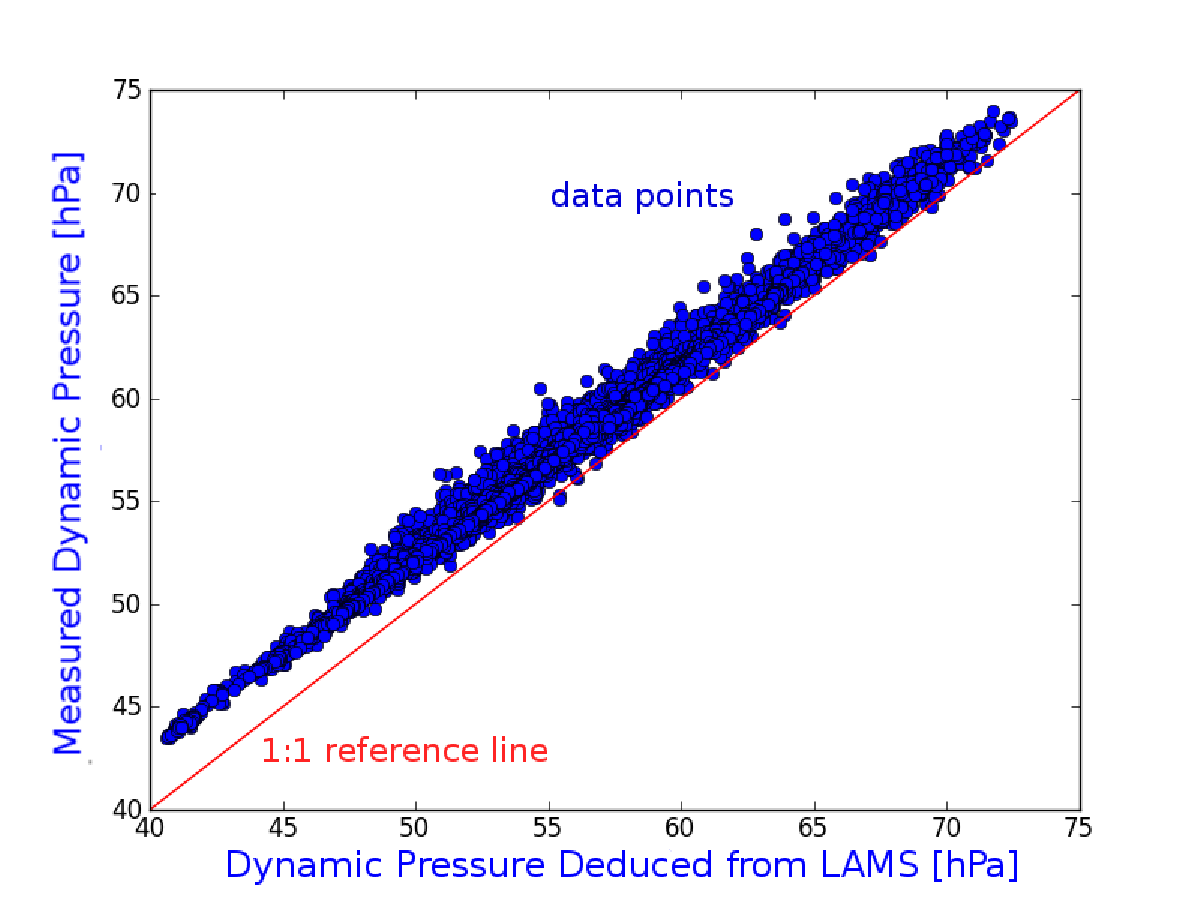
\includegraphics[width=0.9\columnwidth]{Fig1}
\par\end{centering}

\caption{\label{fig:QvsQLAMS-1}The direct measurement of dynamic pressure
($q_{m})$ on the C-130 vs that deduced using the LAMS measurement
of airspeed, via Eqs.~(\ref{eq:PCOR1-1}) and (\ref{eq:PCOR2-1}).
All one-second-average points from one C-130 research flight on which
the LAMS was tested (17 November 2011) are shown.}
\end{figure}


\begin{figure}[H]
\begin{centering}
\vspace*{2mm}

\par\end{centering}

\noindent \begin{centering}
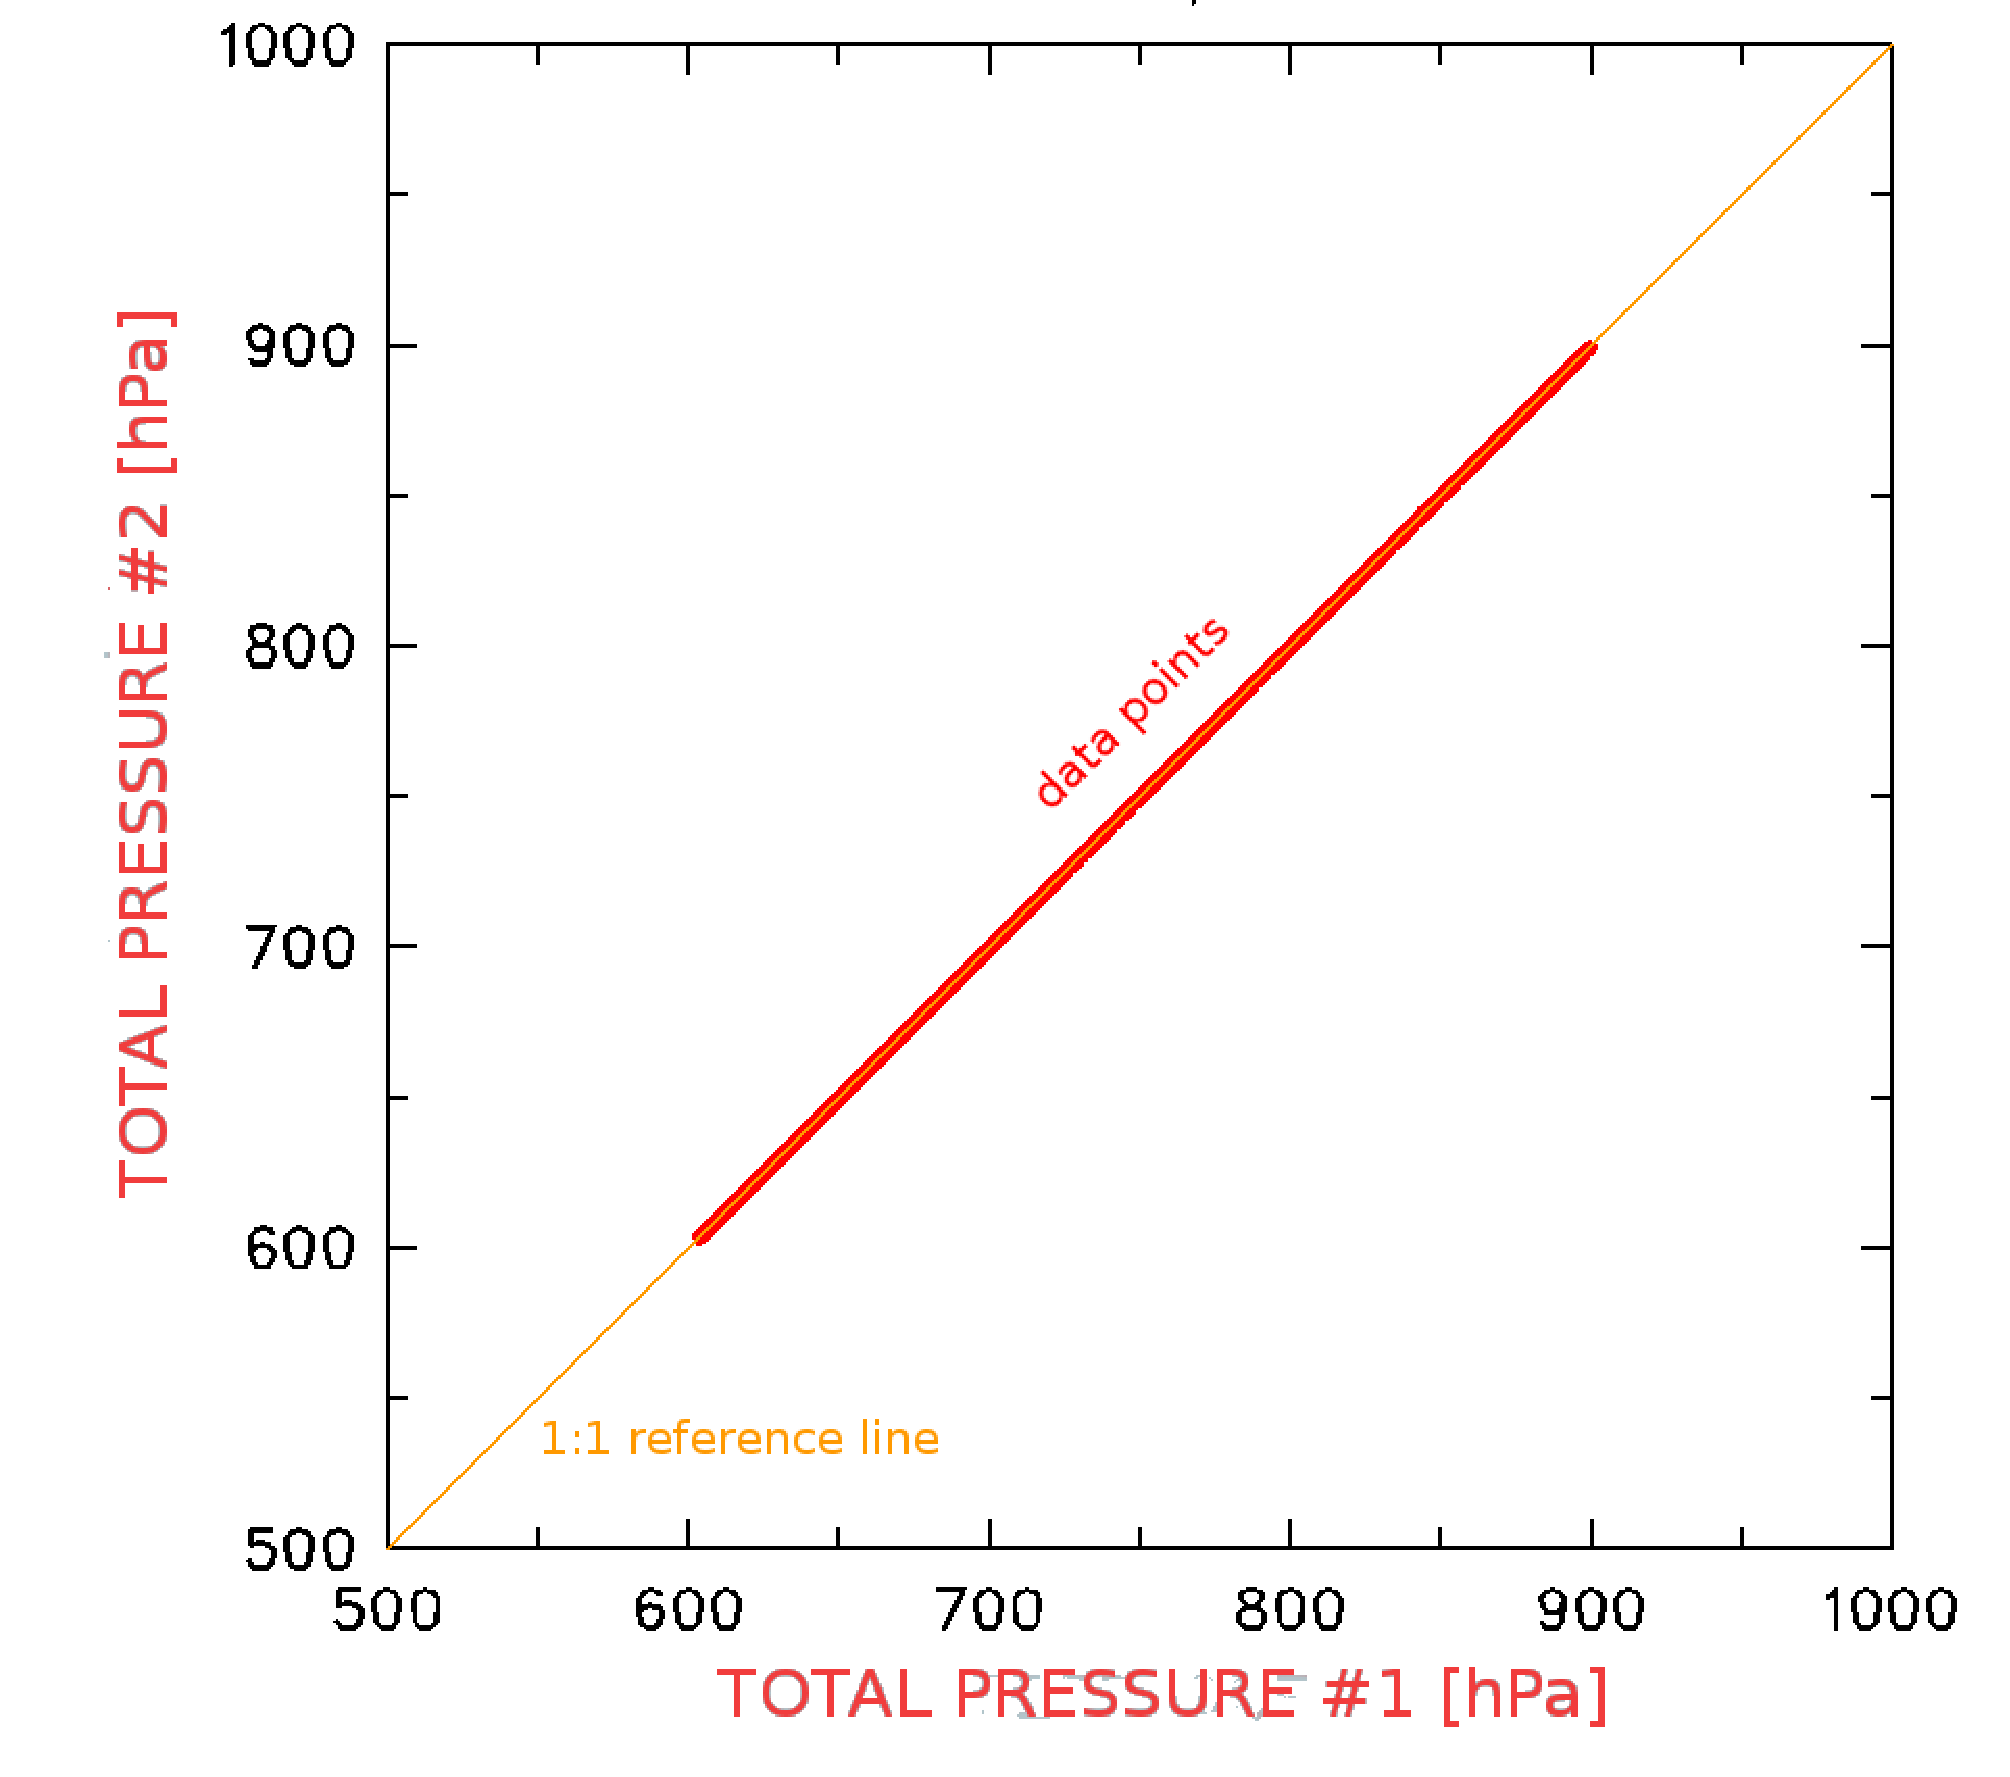
\includegraphics[height=0.6\paperheight]{Fig2}
\par\end{centering}

\caption{\label{fig:Pt-comparison-1}Measurements made at 1\,Hz during the
17 November 2011 flight of the C-130. All measurements are included
for times when the true airspeed exceeded 50\,$\unit{m\,s^{-1}}$
(to exclude a short period with flaps deployed at the end of the flight).
The measurements plotted are the total pressure $p_{t}$ measured
by two independent systems using two different pitot tubes and sets
of static buttons. The root-mean-square deviation from this line is
0.1\,hPa, and the similar deviation from a best-fit line is less
than 0.04\,hPa.}
\end{figure}


\begin{figure}[H]
\noindent \begin{centering}
\vspace*{2mm}
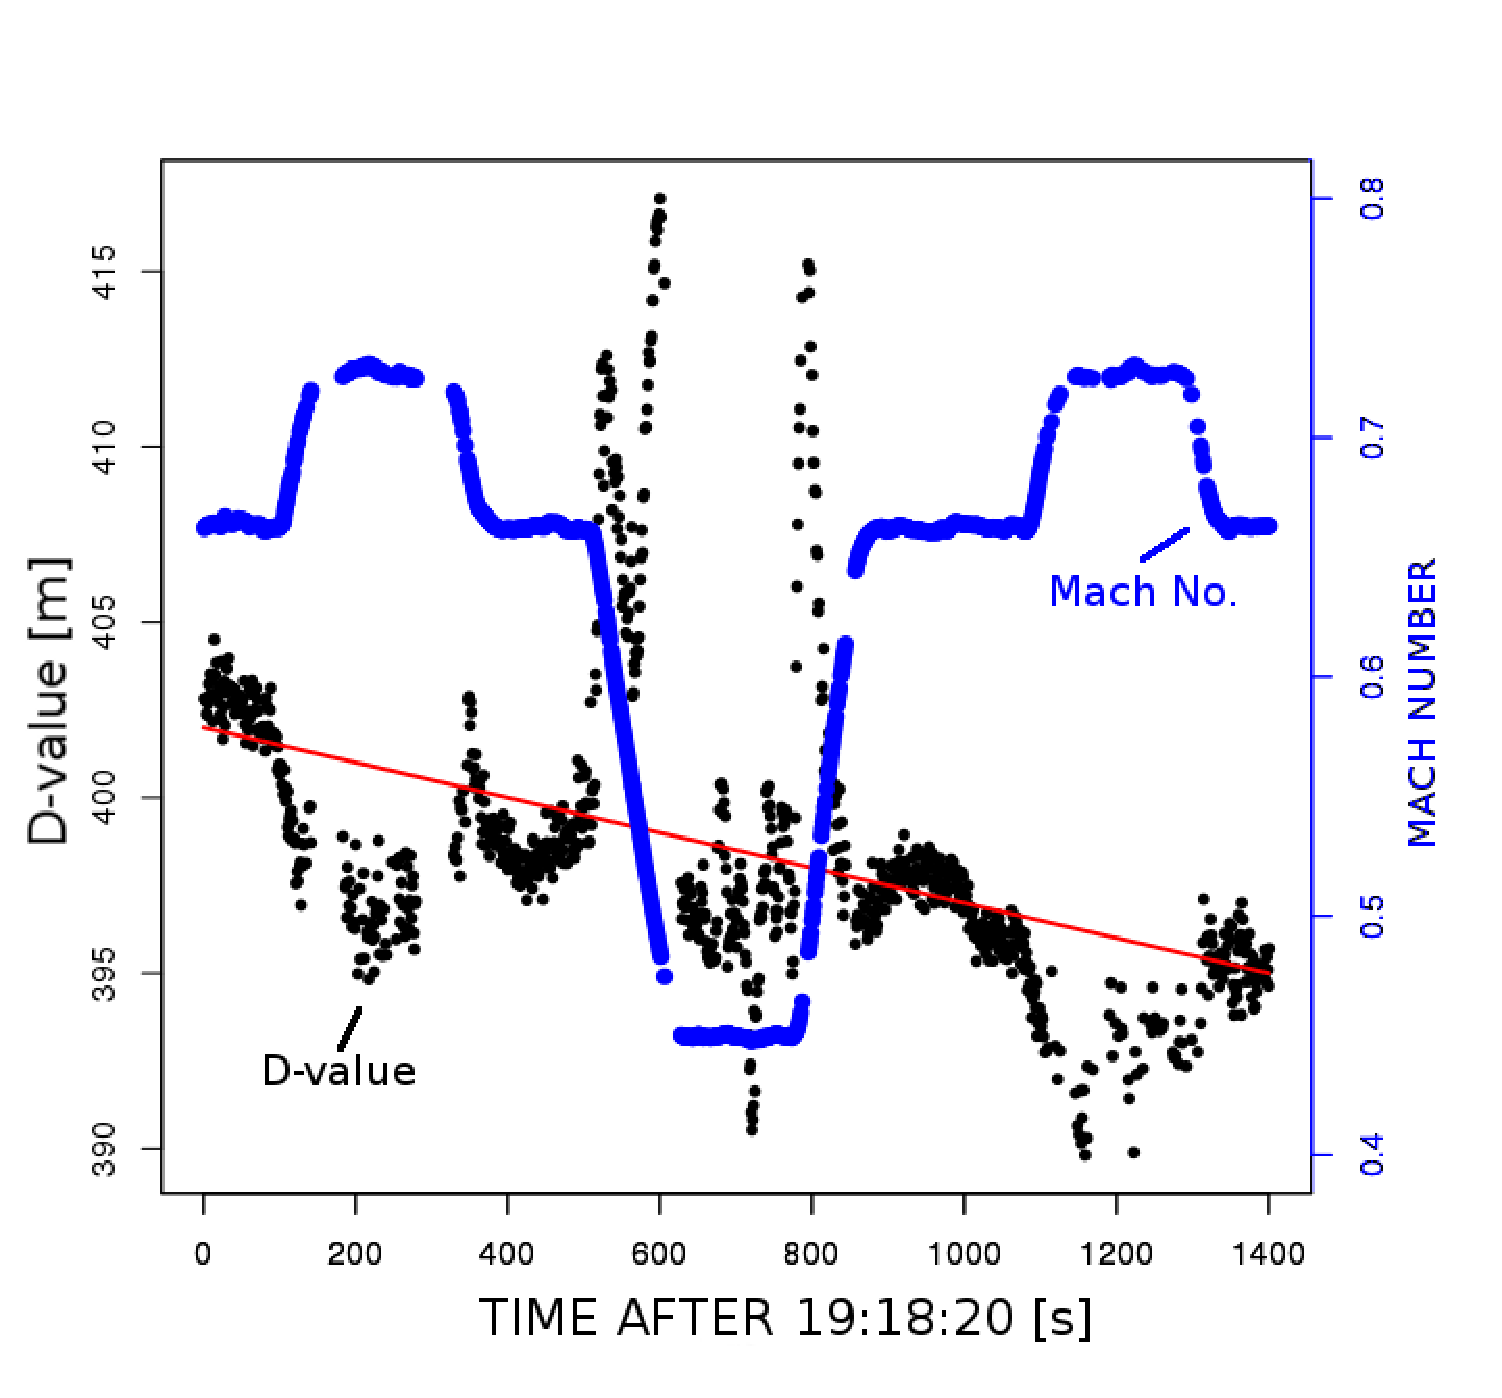
\includegraphics[height=0.65\paperheight]{Fig3}
\par\end{centering}

\caption{\label{fig:D-value-measurements-1}D-value measurements as a function
of time for a flight segment at about 450\,hPa, and the corresponding
values of the Mach number (plotted relative to the right axis). It
might be expected that the d-value would change smoothly, as suggested
by the solid red line. GV flight of 12 August 2010, Colorado USA to
St. Croix, Virgin Islands. Gaps in data show portions omitted because
the LAMS signal was too weak to be reliable.}
\end{figure}


\begin{figure}[H]
\noindent \begin{centering}
\vspace*{2mm}
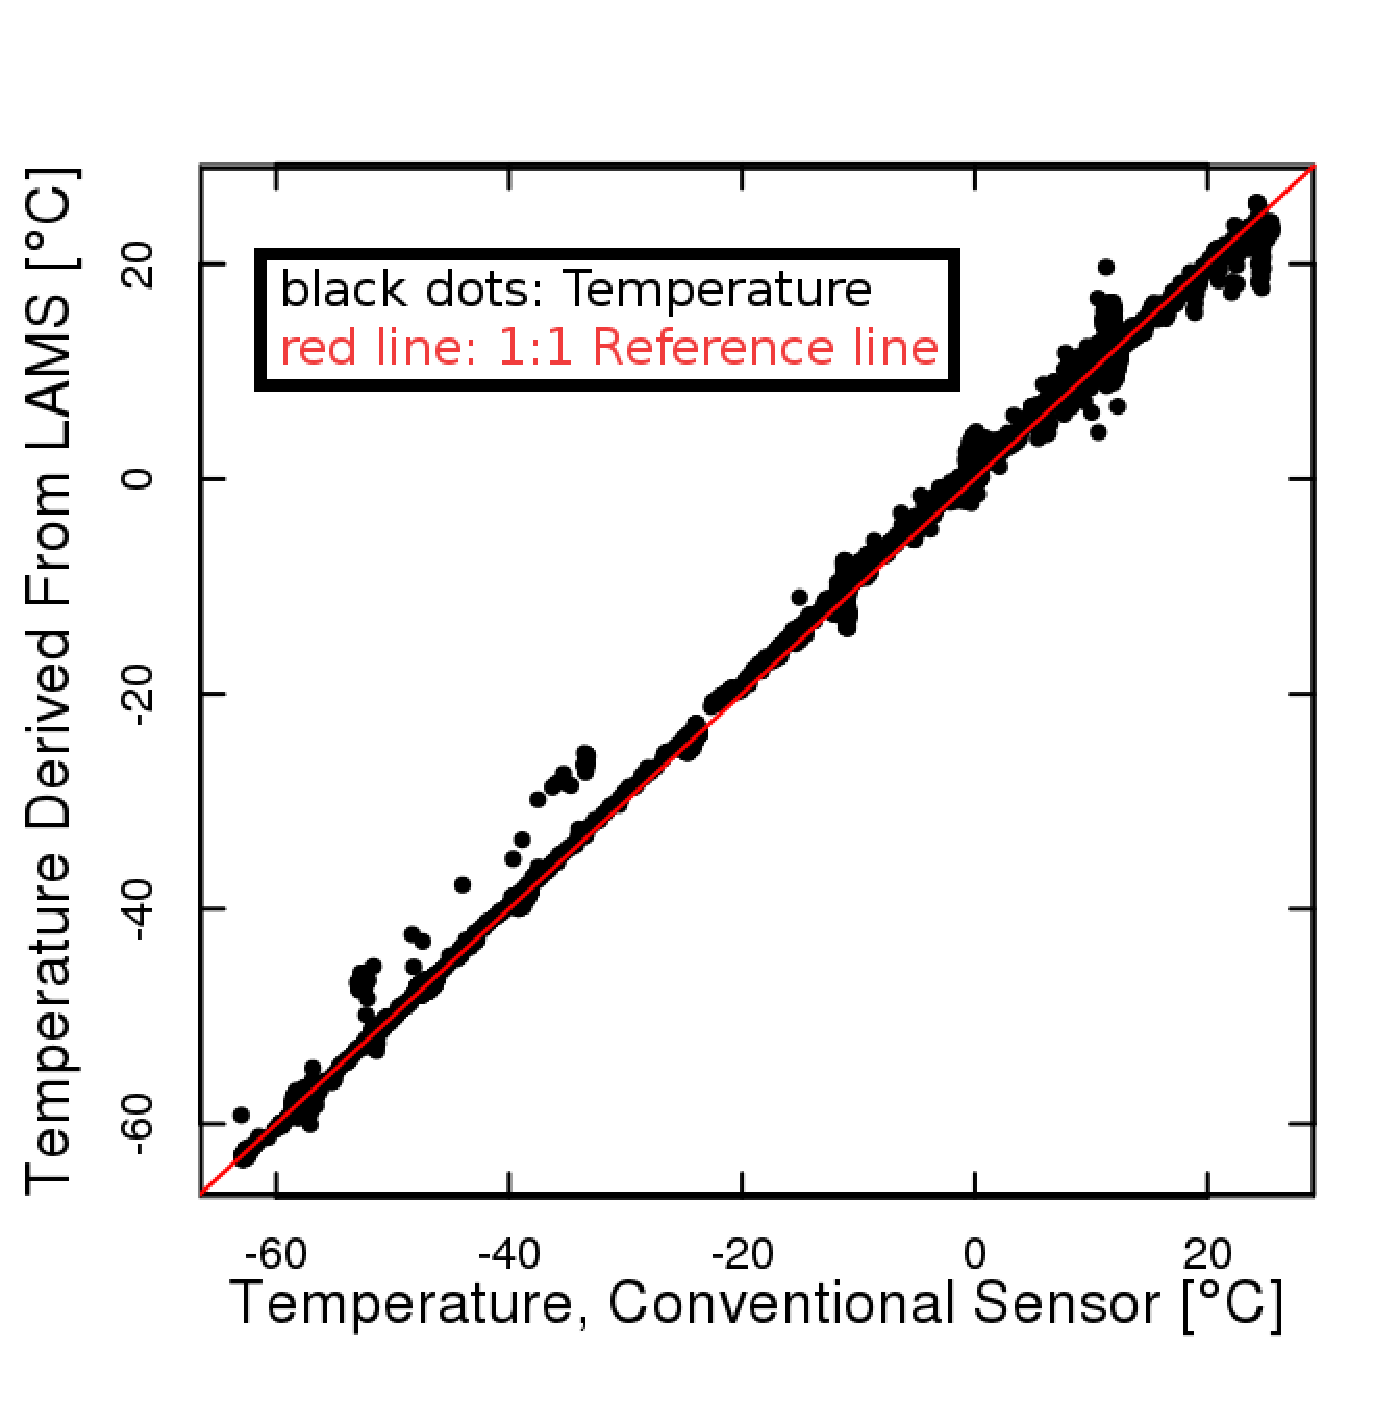
\includegraphics[height=0.6\paperheight]{Fig4}
\par\end{centering}

\caption{\label{fig:ATL-1}Temperature determined from LAMS using (\ref{eq:TfromVL-1})
plotted as a function of the corresponding direct measurement of temperature
for the ferry flight from Colorado USA to St.~Croix, Virgin Islands,
on 10 August 2010. Each plotted point represents a measurement over
one second of flight. }
\end{figure}


\begin{figure}[H]
\noindent \begin{centering}
\vspace*{2mm}
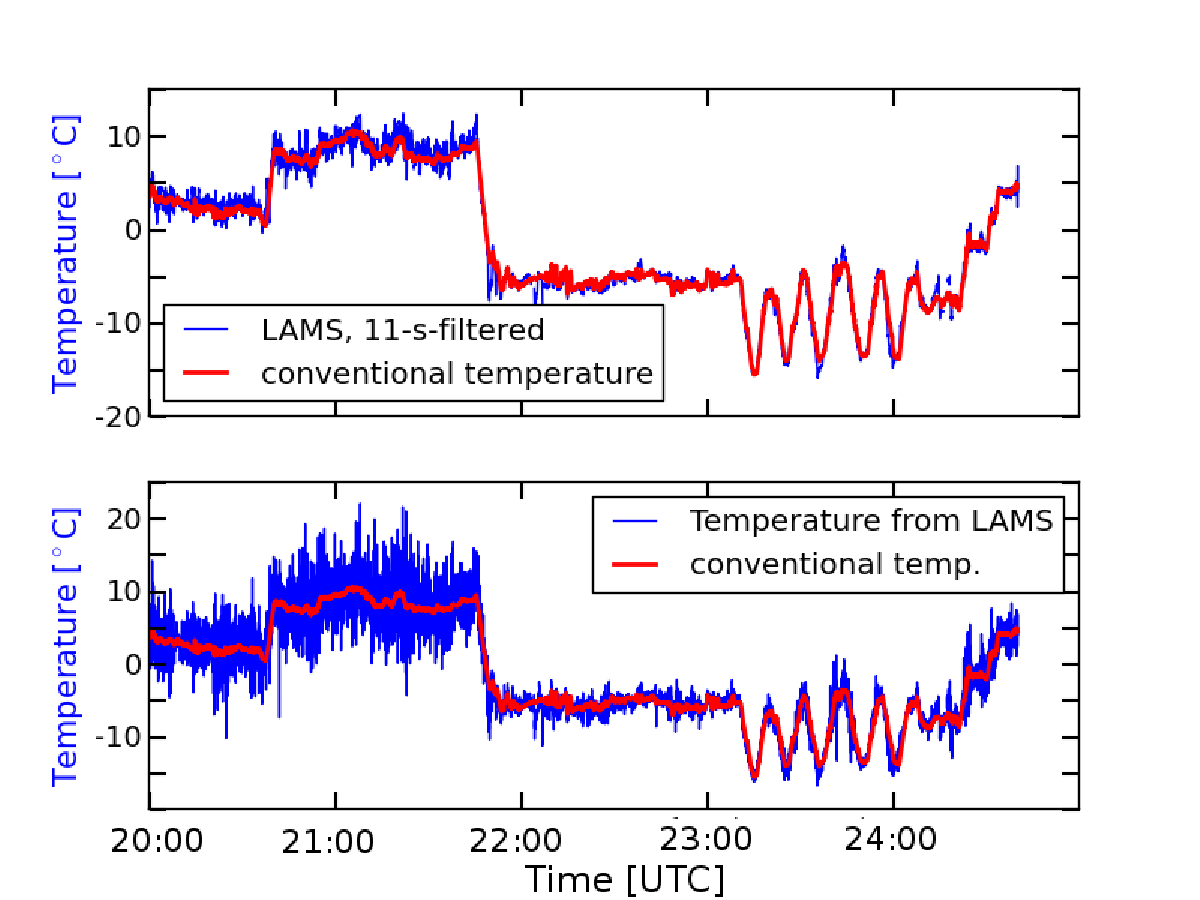
\includegraphics[width=0.9\columnwidth]{Fig5}
\par\end{centering}

\caption{\label{fig:TLAMSvsATX-1}Temperature determined from LAMS plotted
with the standard measurement of temperature for a flight segment
from the C-130 flight of 17 November 2011. The bottom panel shows
the 1-Hz measurements from LAMS; in the top panel, these have been
smoothed by an 11-s box average.}
\end{figure}


\begin{figure}[H]
\noindent \begin{centering}
\vspace*{2mm}
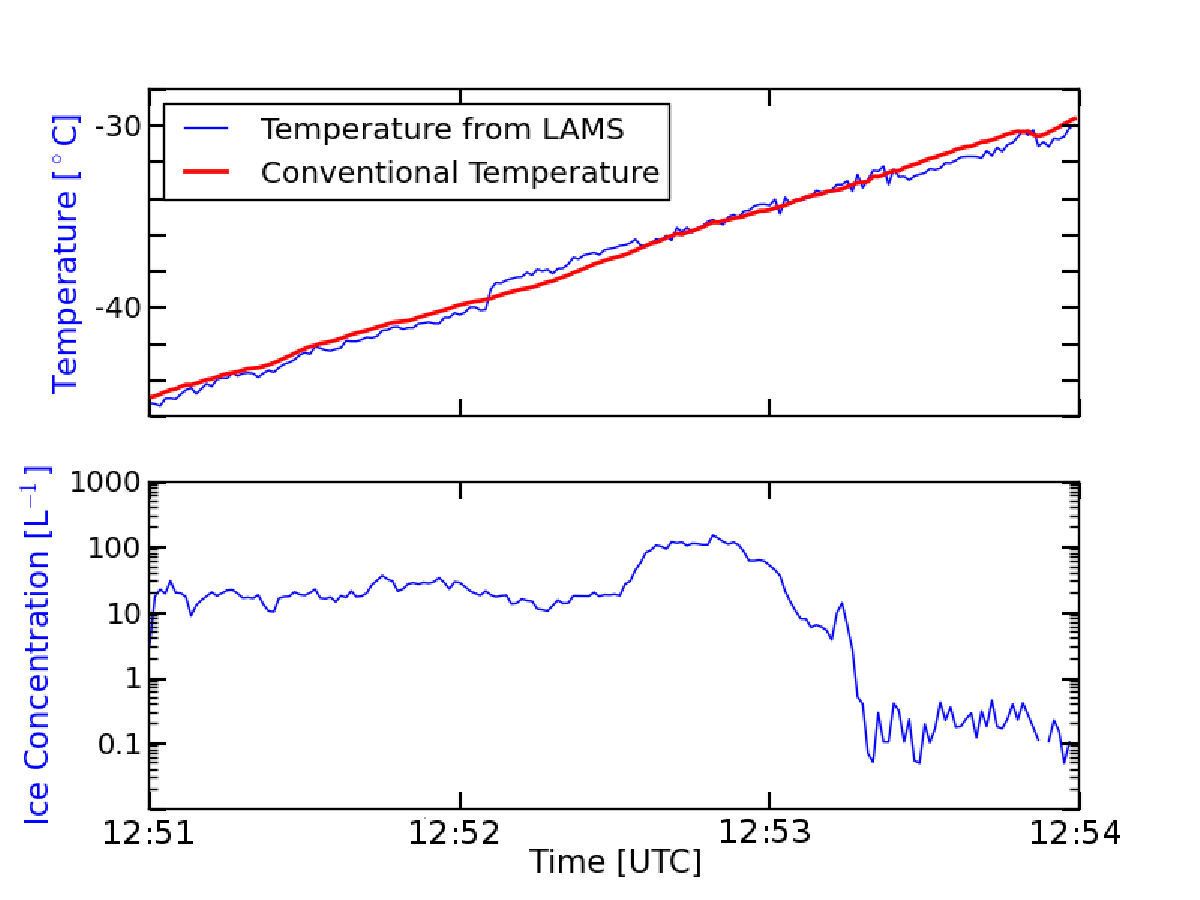
\includegraphics[width=0.9\columnwidth]{Fig6}
\par\end{centering}

\caption{\label{fig:ATLinCirrus-1}Top panel: Temperature determined from LAMS
measurements of airspeed using Eq.~(\ref{eq:TfromVL-1}), compared
to the temperature measured by a conventional immersion temperature
sensor during a descent through a cirrus cloud layer. Bottom panel:
The measured ice concentration from a two-dimensional cloud (2DC)
imaging probe.}
\end{figure}


\begin{figure}[H]
\noindent \begin{centering}
\vspace*{2mm}
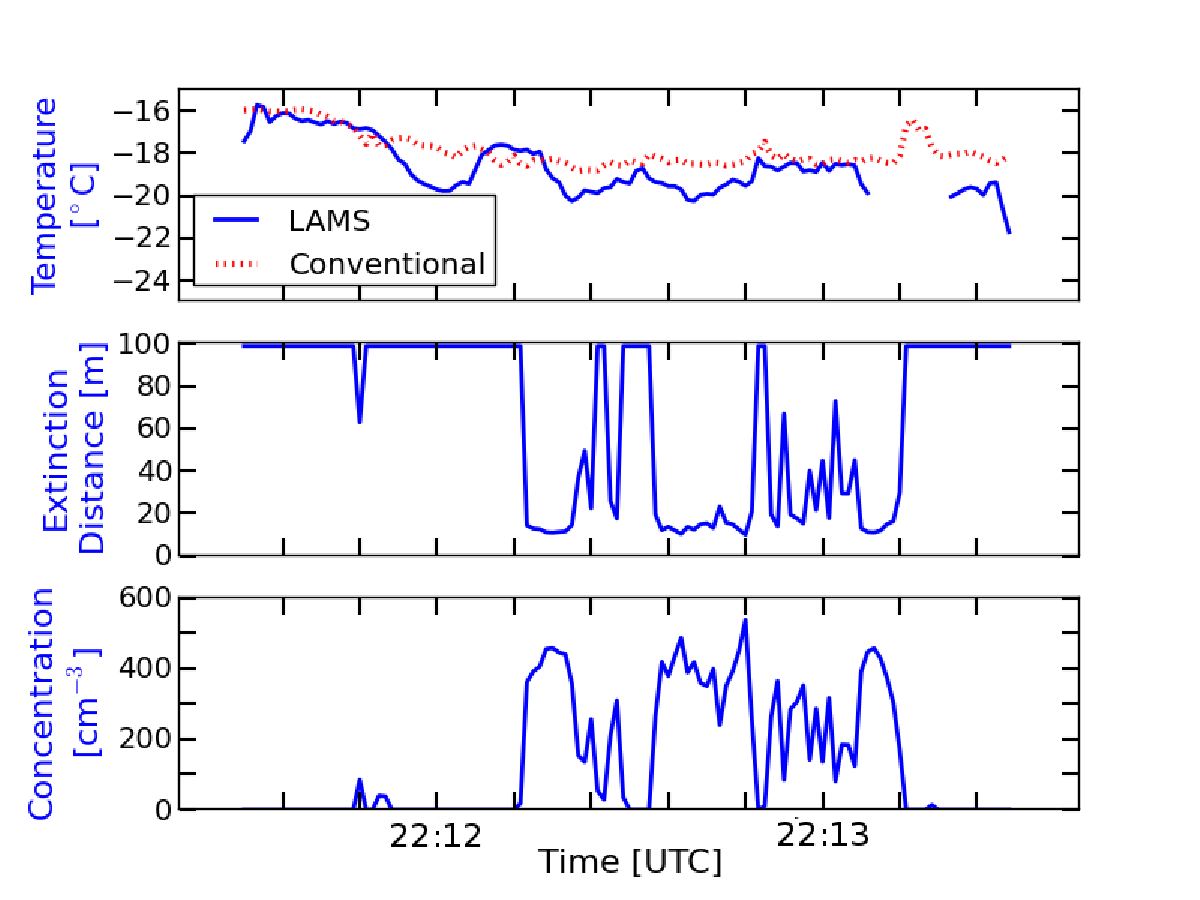
\includegraphics[width=0.9\columnwidth]{Fig7}
\par\end{centering}

\caption{\label{fig:ATLinWaterCloud-1}Top panel: Temperature determined by
the LAMS during a C-130 cloud pass on 15 November 2011. The temperature
measured by a conventional temperature probe is also shown. Middle
panel: Extinction length or distance corresponding to unity optical
depth, determined from the measured droplet size distribution. Bottom
panel: Cloud droplet concentration measured by a cloud droplet probe. }
\end{figure}


\setcounter{figure}{0}%

\def\thefigure{\thesection 1}\def\thefigure{B1}

\appendix\addtocounter{section}{1}
\begin{figure}[H]
\noindent \begin{centering}
\vspace*{2mm}
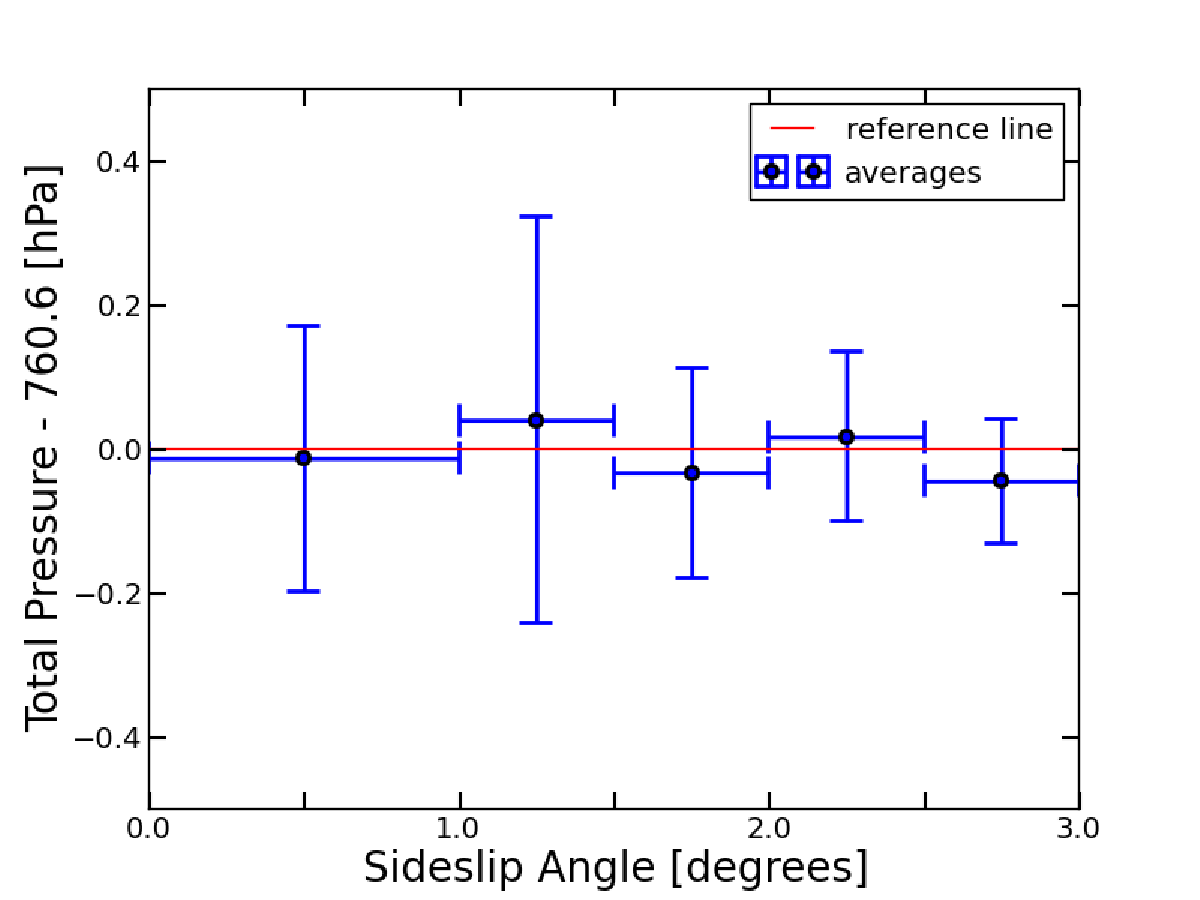
\includegraphics[height=0.6\paperheight]{FigB1}
\par\end{centering}

\caption{\label{fig:PtvsSSLIP-1}The total pressure (from the sum of the ambient
pressure measurement and the dynamic pressure measurement) on the
C-130 as a function of the magnitude of the side-slip angle during
yaw manoeuvres in which sideslip angles were forced by rudder action
while the aircraft continued on approximately a straight-and-level
course. The mean total pressure of 760.6\,hPa has been subtracted
from the measurements. Error bars are standard deviations in the measurements
for the total-pressure axis and are the range of the bin used in sideslip.
Corrections for deviations from a level course and for small variations
in airspeed have been applied, as discussed in the text. }
\end{figure}

\end{document}
